% \documentclass{vldb}
\documentclass[sigconf]{acmart}
\AtBeginDocument{%
  \providecommand\BibTeX{{%
    \normalfont B\kern-0.5em{\scshape i\kern-0.25em b}\kern-0.8em\TeX}}}

\setcopyright{acmcopyright}
\copyrightyear{2018}
\acmYear{2018}
\acmDOI{10.1145/1122445.1122456}

\acmConference[Woodstock '18]{Woodstock '18: ACM Symposium on Neural
  Gaze Detection}{June 03--05, 2018}{Woodstock, NY}
\acmBooktitle{Woodstock '18: ACM Symposium on Neural Gaze Detection,
  June 03--05, 2018, Woodstock, NY}
\acmPrice{15.00}
\acmISBN{978-1-4503-XXXX-X/18/06}

\usepackage[utf8]{inputenc}

\usepackage{graphicx}
\usepackage{url}
\usepackage{multirow}
\usepackage{array}
\usepackage{hyperref}
\usepackage{algorithm} % for algorithms
% \usepackage{algorithmicx}
% \usepackage{algorithm2e} % for algorithms
\usepackage{algpseudocode}
% \usepackage{booktabs} % For formal tables
\algdef{SE}[SUBALG]{Indent}{EndIndent}{}{\algorithmicend\ }%
\algtext*{Indent}
\algtext*{EndIndent}

\usepackage{balance}  % for  \balance command ON LAST PAGE  (only there!)
\usepackage{caption}
\usepackage{subcaption}
\usepackage{tikz}
\usepackage[flushleft]{threeparttable}
\usetikzlibrary{backgrounds, calc, positioning, fit, decorations.pathreplacing}
% \theoremstyle{remark}

\pagestyle{empty} % removes running headers

\newcommand{\PicScale}{0.5}
\newcommand {\FlameStream} {FlameStream}
\newcommand {\tracker} {trAcker}
\newcommand {\acker} {Acker}

\newtheorem{lemma}{Lemma}

% Include information below and uncomment for camera ready
% \vldbTitle{Substream Management in Distributed Streaming Dataflows}
% \vldbAuthors{Artem Trofimov, Nikita Sokolov, Igor Kuralenok, Nikita Marshalkin, and Boris Novikov}
% \vldbDOI{https://doi.org/10.14778/xxxxxxx.xxxxxxx}
% \vldbVolume{12}
% \vldbNumber{xxx}
% \vldbYear{2019}

\begin{document}

\title {Substream Management in Distributed Streaming Dataflows}

\author{Artem Trofimov}
\email{tyoma@lzy.ai}
\affiliation{
  \institution{lzy.ai}
  \city{Tel Aviv}
  \country{Israel}
}

\author{Nikita Sokolov}
\email{faucct@gmail.com}
\affiliation{
  \institution{Yandex Cloud}
  \city{Saint Petersburg}
  \country{Russia}
}

\author{Nikita Marshalkin}
\email{marnikitta@gmail.com}
\affiliation{
  \institution{No affiliation}
  \city{Limassol}
  \country{Cyprus}
}

\author{Igor Kuralenok}
\email{igor.kuralenok@huawei.com}
\affiliation{
  \institution{Huawei}
  \city{Saint Petersburg}
  \country{Russia}
}

\author{Boris Novikov}
\email{borisnov@acm.org}
\affiliation{
  \institution{HSE University}
  \city{Saint Petersburg}
  \country{Russia}
}

% \numberofauthors{5}
% Nikita Sokolov\\
%     \affaddr{Yandex}\\
%     \affaddr{Saint Petersburg, Russia}\\
%     \email{faucct@yandex-team.ru}
% \alignauthor
% Igor Kuralenok\\
%     \affaddr{Yandex}\\
%     \affaddr{Saint Petersburg, Russia}\\
%     \email{solar@yandex-team.ru}
% \and 
% \alignauthor
% Nikita Marshalkin\\
%     \affaddr{VK}\\
%     \affaddr{Saint Petersburg, Russia}\\
%     \email{n.marshalkin@corp.vk.com}
% \alignauthor
% Boris Novikov\\
%     \affaddr{HSE University}\\
%     \affaddr{Saint Petersburg, Russia}\\
%     \email{borisnov@acm.org}
% }

\begin{abstract}
Most state-of-the-art SPEs use punctuations to divide a stream into bounded substreams of messages, such as epochs and windows. The punctuation approach is powerful but has limitations: it does not support cyclic dataflows, is poorly scalable in some cases due to intensive use of broadcasts, and becomes inefficient when the number of chunks or cluster size becomes significant. We introduce a new substream tracking technique called \tracker\ that overcomes the limits of punctuations. We experimentally evaluate the properties of \tracker\ in both synthetic and real-world environments. Experiments show that our technique outperforms punctuations for a large number of substreams and efficiently handles real-world cyclic dataflows.
\end{abstract}

\begin{CCSXML}
<ccs2012>
<concept>
<concept_id>10002951.10002952.10003190.10010842</concept_id>
<concept_desc>Information systems~Stream management</concept_desc>
<concept_significance>500</concept_significance>
</concept>
</ccs2012>
\end{CCSXML}

\ccsdesc[500]{Information systems~Stream management}

\keywords{Data streams, punctuations, stream join, state management}

\maketitle

% \keywords{Data streams, exactly-once, drifting state, optimistic OOP}

\thispagestyle{empty}

\section {Introduction}
\label {fs-acker-intro}

Distributed stream processing engines (SPEs), such as Flink~\cite{carbone2015apache}, Heron~\cite{Kulkarni:2015:THS:2723372.2742788}, or MillWheel~\cite{Akidau:2013:MFS:2536222.2536229}, aim to handle potentially unbounded sequences of data elements. These systems receive input elements one-by-one, process them, update the internal state, and eventually release results. 

The processing of unbounded data sequences has at least two difficulties. First, SPEs should be aware of resource consumption: SPE can maintain an in-memory state with no upper bound in size and run out of memory. Second, SPEs observe elements sequentially, but traditional relational operators assume finite data sources with random access. Therefore, to produce correct results, there is a need to determine the ``bounds'' of the query.

In practice, infinite streams are often considered as a mixture of possibly finite substreams to deal with these difficulties. The examples of such scenarios are listed below.

\noindent {\bf State pruning}. Most SPEs group state by processing keys that are used for data partitioning. For example, if the task is to aggregate news about various social events, an event would likely be the key. The problem here is that the state can grow unlimitedly~\cite{Tucker:2003:EPS:776752.776780}. To prevent overflow, SPE can remove state for outdated keys, e.g., for completed events. In this case, we can consider the stream as a mixture of substreams: one per event.  

\noindent {\bf Time windowed aggregations}. One way to produce results for a relational query is to process elements within event time windows. A time window can define a substream. To release output, an SPE needs a guarantee that all data within a time window are received. This method is widely applied in online analytics~\cite{traub2018scotty} and is used for streaming SQL implementation~\cite{Begoli:2019:OSR:3299869.3314040}.

\noindent {\bf State snapshotting}. Epoch-based state snapshotting is a popular recovery technique applied in Flink~\cite{Carbone:2017:SMA:3137765.3137777}, Storm~\cite{Toshniwal:2014:STO:2588555.2595641}, Samza~\cite{Noghabi:2017:SSS:3137765.3137770}, IBM Streams~\cite{jacques2016consistent}. This method divides all input elements into special substreams called {\em epochs}. An SPE takes a state snapshot when a regular epoch is {\em atomically} processed. In case of failures, SPE can consistently recover state from the snapshot~\cite{2015arXiv150608603C}. 


Each of these scenarios can be considered as a special case of {\em substream management problem}. This problem is to monitor substreams emergence and termination. More formally, a substream is a part of the stream such that all its elements satisfy some predicate. For example, in the case of state pruning, the predicate is {\em [a data element contains key $X$]}, while for time window aggregations, the predicate is {\em [a data element is generated with timestamp less than $T$]}. 

Substreams can be finite or infinite. In this paper, we focus on substreams lifespan monitoring, so we consider finite substreams only. Note that various properties of substream termination events may be required by practical problems:
\begin{itemize}
    \item Time windowed aggregations include some special scenarios, e.g., deterministic windowed join, that require an order of signals to be synchronized with the order of input elements (termination events from data producers)~\cite{najdataei2019stretch, gulisano2016scalejoin}.
    \item Epoch is a substream that an SPE should atomically process. Therefore, the epoch termination event should be received before any elements from the next epoch~\cite{2015arXiv150608603C}. 
    \item State pruning problem does not require any specific properties from termination events. However, high latency between the actual substream termination (the event from data producer) and termination event receiving may reduce the efficiency of a substream management technique.
\end{itemize}

A popular substream management method is punctuations framework~\cite{tucker2003exploiting}. The main idea behind this framework is to divide the stream into substreams by injection of particular elements called {\em punctuations} that define substreams ``borders''. While the punctuations approach is robust and easy-to-implement, it has two limitations. First, it does not support general cyclic dataflows~\cite{carbone2018scalable}. Second, the ``border'' elements are frequently broadcasted between SPE nodes, so punctuations have high network traffic overhead and can reduce the throughput of an SPE for small substreams~\cite{Li:2008:OPN:1453856.1453890}. 

In this work, we introduce a new substream management framework called \tracker. Within this framework, we introduce an additional agent (process) that receives information about substreams from an SPE and sends back substream lifespan events. This way, the substream lifespan events are propagated through this agent, allowing SPE to reduce network traffic overhead significantly. Such propagation method is suitable for cyclic dataflows because service traffic does not go through the cycles.

By tackling these challenges, \tracker\ opens an ability to apply substreams-based techniques for new applications, such as iterative stream processing, and new setups, e.g., very granular substreams. We compare the performance of \tracker\ to the punctuations framework applied in most state-of-the-art SPEs. We demonstrate that \tracker\ outperforms punctuations on synthetic and real-world dataflows. We also show a novel application of the substream management for a real-world cyclic dataflow. 

As we can see, substream management problem appears in many practical scenarios. Moreover, the properties of some substreams impose requirements on the substream termination events. We formalize the substream management problem and generalize its properties. It allows us to ensure that our approach is suitable for the mentioned scenarios as well as for the more general problems that require substream management.

In summary, our contributions are as follows:
\begin{enumerate}
    \item We provide a formal model of substream management. This model allows us to compare the properties of various substream management systems.
    \item We present a novel substream management technique that achieves a lower bound of network traffic overhead.
    \item We demonstrate \tracker\ performance in comparison to a state-of-the-art approach on diverse workloads.
\end{enumerate}

The rest of the paper is organized as follows: Section~\ref{fs-acker-preliminaries} formalizes the substream management problem and indicates the main properties of a solution. In Section~\ref{fs-acker-tracker}, we introduce a general design of the \tracker\ framework and demonstrate that it satisfies the formal properties of the substream management solution. Section~\ref{fs-acker-impl} summarizes the implementation of \tracker\ for both centralized and distributed setups with optimizations that can reduce the amount of extra traffic. In Section~\ref{fs-experiments}, we show that the proposed technique is scalable and can outperform alternatives employed in state-of-the-art stream processing engines. The relevant prior research is outlined in Section~\ref{fs-acker-related}. Finally, we discuss our conclusions in Section~\ref{fs-acker-conclusion}.

\section{Substream management}
\label{fs-acker-preliminaries}

First, in this section, we formalize the notion of a stream processing engine, based on Chandy-Lamport definition of a distributed system and build specifics needed for stream processing on top of this model. Then we introduce substream lifespan management, based on events from the proposed model. Fnally we study what properties of the introduced    technique are needed for practical applications.

\subsection{Processing model}

\begin{figure}[htbp]
  \centering
  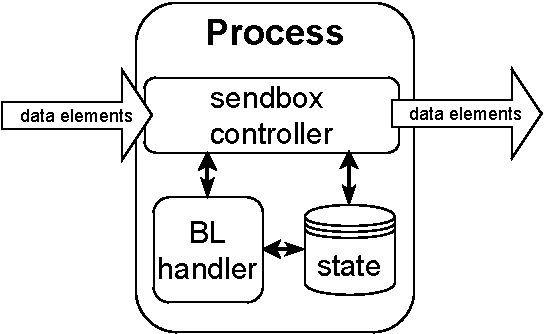
\includegraphics[width=0.50\textwidth]{pics/process-scheme.pdf}
  \caption{Structure of the SPE process}
  \label{fig:spe_process}
\end{figure}

Typically, distributed stream processing engines are shared-nothing runtimes that continuously ingest input elements, transform them according to a logical dataflow graph, and deliver output elements. The logical dataflow graph consists of user-defined operators. Operators can be stateless or stateful: an output element may depend on the current state and the corresponding input element. A logical graph is mapped to a physical, distributed graph upon deployment. Commonly, a single logical operator can be deployed on multiple computational nodes. Further, we denote physical instances of logical operators as {\em processes}.

A deployed physical graph is a distributed system and could be described in terms of Chandy-Lamport model~\cite{lamport}. In this model authors introduce \textit{events} that allows to observe a state of the system. Each event is presented in tuple of 5 elements $e = (p, s, s', c, M)$, where $p$ is one of the deployed processes, $s$ and $s'$ are state of the process before and after processing, $c$ one of network FIFO channels that connect processes with each other, and $M$ is a message generated during processing. The generated event $M$ come to a channel state $C$ until it will be received by destination process. Processes and channels forms a physical graph of the system $G=\{\Pi,\mathcal{E}\}$.

In a stream processing engine we need to specify a process $p$ to reflect a specifics of this type of processing. Besides user-defined state each SPE process has a special storage for messages. We call this storage \textit{sendbox} $B_p$. This storage is needed for many reasons as will be discussed later in the paper. Here we justify the existence of \textit{sendbox} by necessity to send multiple events from one user-defined model to multiple recipients which contradicts with the original model. To manage the sendbox SPEs have a special agent. In our model we extend a role of this agent to inject a substream management there. Find a schematic representation of the model in Fig.~\ref{fig:spe_process}.

With the specified process we need to introduce special cases of system events:
\begin{itemize}
    \item Communication events: $recv$, $send$, these events are executed by sendbox controller
    \item Processing events: user-defined procedures are isolated here
    \item System events: consistency, substreams and other events in the system that provide its properties
\end{itemize}

Communication events are straightforward: $<recv, M> = (sendbox\_controller_p, B_p, B_p' = B_p\cup \{M\}, c_qp, M)$, $<send, M> = (sendbox\_controller_p, B_p, B_p' = B_p\setminus\{M\}, c_{p, dst(M)}, M)$. Note that we need to be able to get destination process directly from the message and in general message contains its source and destination, this allows us to abstract away from the physical channels which are unknown to the user-defined procedure that emits the event. As a practical case of this abstraction is a sharding scheme for some key: user-defined procedure emits event for some key and a system is responsible to find a proper physical channel to deliver this message.

Processing events are triggered by a process and allows to execute user-defined logic with the events provided by sendbox controller. Please note, that these events does not communicate with other processes and are isolated in the state of the SPE process. $<proc, M> = (func_p, s\setminus M, s \cup \{func_p(M)\}, null, null>$.

System events set depends on the system and will be defined latter in the description of particular implementation.

Note that all events within the same process $p$ are totally ordered by a local causal order relation $<_p$: $e^{0}_p,e^{1}_p,...,e^{i}_p,...$. Atomicity of the events and their sequential nature allows a system to build guaranties for processing and state management.

\subsection{Predicates on system events}
As stated in the introduction we want to allow a user or a system itself to define predicates for events in the system, track their values for all messages in the system ($S = C \cup \cup_p B_P$) . This will give opportunity to define and track quantifier expressions, that could be basis of guarantee mechanisms.

\subsubsection{Soft bound}

Many applications that apply substream management systems do not require any special properties of termination events. In this case, we denote the guarantee provided by such events as {\em soft bound}, because termination events indicate only the fact that the substream ended some time ago, and other input elements could be processed after that. More formally, we define the soft bound guarantee of the termination event (end-of-substream) $\langle eoss_{soft}, pred(m)\rangle$ as follows:

\begin{align*}
\forall e^{'} = \langle proc,m\rangle, e^{'} >_p \langle eoss_{soft}, pred(m)\rangle : \neg pred(m)
\end{align*}

Figure~\ref{general_guarantees} illustrates this notion. Terms $a,b,c,d...$ denote ordered processing events of a process $p$. The substream ends after event $c$. Note that there are several other events between the end-of-substream and $c$. This is the property of a {\em soft bound} guarantee: if $\langle eoss, pred(m)\rangle$ occurs, all subsequent elements do not satisfy the predicate, but it is not necessarily the exact substream ``border''.

\begin{figure}[htbp]
  \centering
  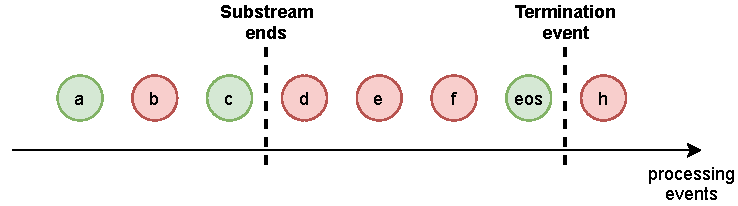
\includegraphics[width=0.50\textwidth]{pics/general-guarantee.pdf}
  \caption{Substream management: soft bound}
  \label{general_guarantees}
\end{figure}

\subsubsection{Firm bound}

The guarantee that any new event will not satisfy the predicate is sufficient for many real-life problems, e.g., SPE can initiate process state pruning on such events. However, some problems require a {\em firm bound}: guarantee that the substream ends {\em exactly} after the termination event. 

For example, epoch-based snapshotting protocol~\cite{2015arXiv150608603C, jacques2016consistent} bases on a notion of {\em epoch}. Epoch is a special substream that should be atomically processed. Therefore, SPE requires the termination event for an epoch that occurs right after the last processing event for this epoch. Otherwise, the snapshot can be inconsistent, because it captures elements from various epochs. To support such scenarios, the end-of-substream event $\langle eoss_{firm}, pred(m)\rangle$ should satsify the following conditions:

\begin{align*}
&1. \forall e^{'} = \langle proc,m\rangle, e^{'} >_p \langle eoss_{firm}, pred(m)\rangle : \neg pred(m) \\
&\boldsymbol{2. \forall e^{*} = \langle proc,m\rangle, e^{*} <_p \langle eoss_{firm}, pred(m)\rangle : pred(m)} \\
\end{align*}

The first condition is the same as for the soft bound guarantee. The second one allows a process to determine the exact processing event when the substream terminates: all elements after the termination event will not satisfy the predicate, but all previous elements have been satisfied. 

Figure~\ref{strict_guarantees} illustrates the notion of the firm bound. As in the previous example, terms $a,b,c,d...$ denote ordered processing events of a process $p$. However, in this case, event $\langle eoss_{firm}, pred(m)\rangle$ occurs right after the substream terminates.

\begin{figure}[htbp]
  \centering
  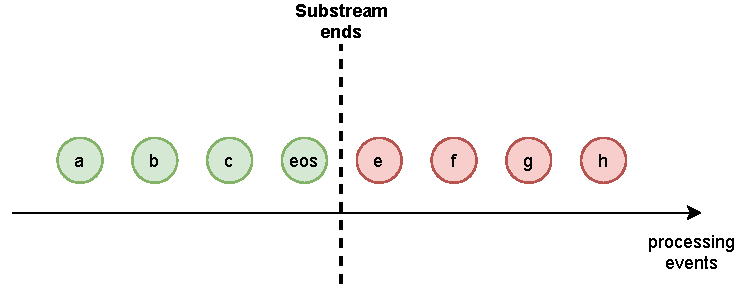
\includegraphics[width=0.50\textwidth]{pics/strict-guarantee.pdf}
  \caption{Substream management: firm bound}
  \label{strict_guarantees}
\end{figure}

\subsubsection{Consistent termination events order}
Some specific applications, including the mentioned earlier epoch-based snapshotting method and techniques for enforcing deterministic processing~\cite{we2018adbis} require an order of termination events to be synchronized with the order of substreams endings (events from data sources). For example, if termination events are reordered, then snapshots for consecutive epochs can be inconsistent. Another example is deterministic join that also requires the defined order of termination events~\cite{gulisano2016scalejoin}.

\begin{figure}[htbp]
  \centering
  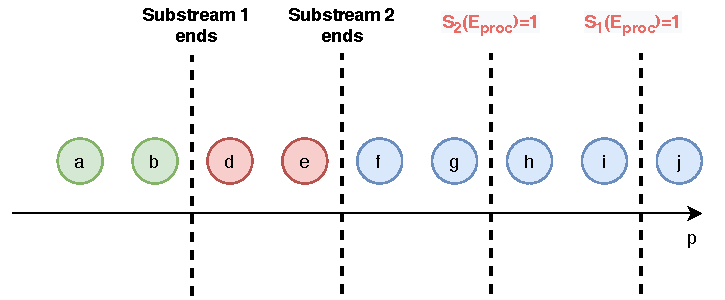
\includegraphics[width=0.50\textwidth]{pics/notifications-reordering.pdf}
  \caption{An example of termination events reordering}
  \label{notifications_reordering}
\end{figure}

Termination events reordering in case of the soft bound guarantee is illustrated in Figure~\ref{notifications_reordering}. Terms $a,b,c,d...$ denote ordered processing events of a process $p$. Although the substream containing events $a,b$ terminates earlier, the end-of-substream event for this substream occurs after the termination event for the substream containing events $d,e$. 

Let $e^{*}_1$ and $e^{*}_2$ be the last elements of substreams defined by predicates $pred_1(m)$ and $pred_2(m)$. Termination events $\langle eoss, pred_1(m)\rangle$ and $\langle eoss, pred_2(m)\rangle$ are {\em consistently ordered} iff:

\begin{align*}
e^{*}_1 >_p e^{*}_2 \Longrightarrow \langle eoss, pred_1(m)\rangle >_p \langle eoss, pred_2(m)\rangle
\end{align*}

\subsection{Punctuations framework}

\subsubsection{Framework overview}

The main idea behind the punctuations framework is to divide the stream into substreams by injection of special elements that bear predicate $punct$. Punctuations are injected directly into a system as ordinary data elements by SPE or by external data producers. The injector promises that all further produced records do not satisfy the predicate. Hence, the punctuation itself defines the ``border'' of a substream.

Figure~\ref{punctuations_scheme} illustrates the punctuations framework. Green elements indicate elements that belong to some substream, while red elements do not. As we can see, punctuations play the role of delimiter between the substream elements and all further items.

\begin{figure}[htbp]
  \centering
  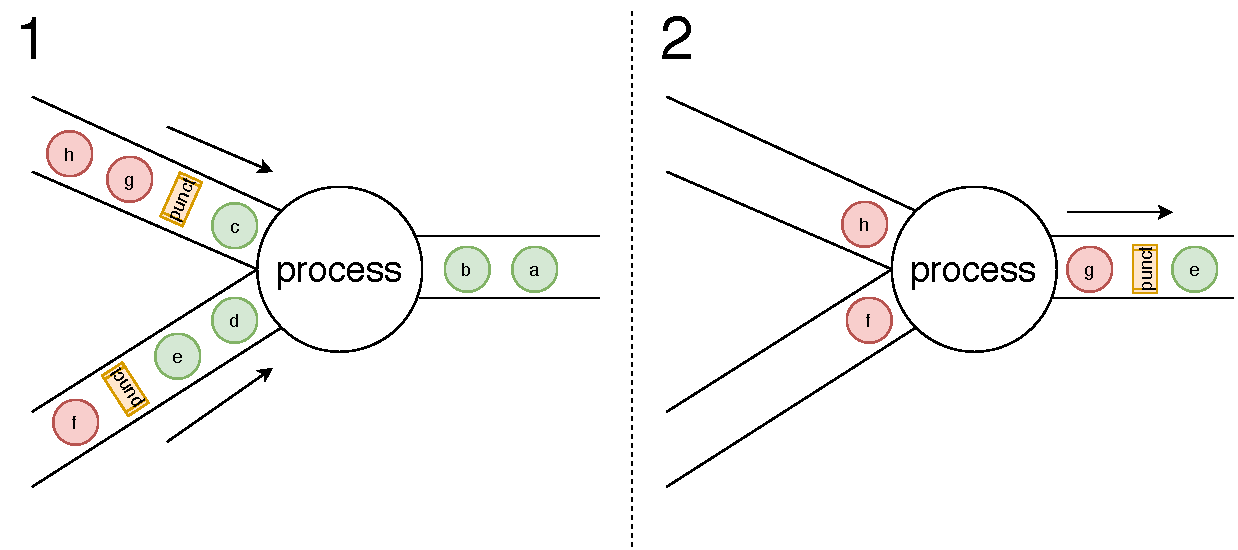
\includegraphics[width=0.50\textwidth]{pics/punctuations-scheme.pdf}
  \caption{Punctuations framework: an example}
  \label{punctuations_scheme}
\end{figure}

Processes within SPE do not apply user-defined operators to punctuations. Instead, each process propagates punctuation to all outgoing channels when it receives corresponding punctuations from all input channels. If a process receives punctuations from all inputs, it is guaranteed that it will not receive elements that satisfy the predicate further due to FIFO network channels. Hence, the formal condition of soft bound termination event $\langle eoss_{soft}, pred(m)\rangle$ is the following:

\begin{align*}
& \langle eoss_{soft}, pred(m)\rangle \Longleftrightarrow \\ 
& \forall q \in I_p, \exists punct_{qp} \in B_p, \forall m\in B : \neg pred(m)
\end{align*}

To satisfy the firm bound guarantee, one needs to hold elements in the sendbox until all punctuations have arrived from all input channels. In~\cite{Carbone:2017:SMA:3137765.3137777} such behavior is called {\em watermark (punctuation) alignment}. More formally, the sendbox procedure should ensure the following order of elements processing to achieve firm bound:

\begin{align*}
& \exists q \in I_p, e = \langle recv,m_{qp} \rangle >_p e^{'} = \langle recv,punct_{qp}\rangle \Longrightarrow \\ 
& <proc, m_{qp}> >_p \langle eoss_{soft}, pred(m)\rangle
\end{align*}

If this condition is satisfied, then $\langle eoss_{firm}, pred(m)\rangle$ = $\langle eoss_{soft}, pred(m)\rangle$ for the punctuations. The punctuations framework provides consistent termination events order by design because punctuations are naturally ordered with ordinary data elements within the processes.

\subsection{Discussion}

\subsubsection{Limitations of punctuations}

While the punctuations approach is robust and easy-to-implement, it has several limitations. In the punctuations framework, the information about the ending of a substream is propagated using ordinary data elements via the data flow network channels. It implies that punctuations are not applicable for cyclic dataflows because a process that receives elements from a cyclic channel will never receive punctuations from this channel~\cite{carbone2018scalable}.

The high network overhead forms another limitation. This method's amount of service traffic is $O(K||\Pi||^2)$, where $||\Pi||$ is the number of processes and $K$ is the number of substreams. As we can see, this estimation is far from the lower bound ($O(||\Pi||)$). It is quadratic in the number of processes, as each process should propagate punctuations to all output channels. 

Substreams can be {\em fine-grained}: for example, each processing key can spawn a substream within a state pruning problem. If there are a lot of small substreams, an inefficient substream management system can reduce the throughput of an SPE itself~\cite{Li:2008:OPN:1453856.1453890} or affect the performance of state checkpointing~\cite{zhang2021research}. As we demonstrate further, the punctuation technique adds significant performance overhead on regular processing for small substreams (frequent punctuations injection).

\subsubsection{Optimal traffic overhead}

A vital performance property of a substream management system is the amount of extra network traffic. Let $||\Pi||$ be a number of processes, and $K$ be a number of substreams. 

\begin{lemma}
The network overhead induced by a substream management system cannot be lower than $O(K||\Pi||)$. 
\end{lemma}
\begin{proof}
When a substream management system detects the end of a substream, it should inform processes about that. In a general case, e.g., for a state snapshotting problem, it should inform all (stateful) processes. Hence, at least one network message (termination notification) must be sent to each process for each substream.
\end{proof}

Despite this lemma's simplicity, we will further use it to figure out how far is some substream management system from this bound. We can also claim a solution as {\em optimal} if its extra traffic estimation is equal to the lower bound from the lemma. In the next sections, we demonstrate that it is possible to design a substream management system that achieves optimal network traffic overhead.


\section{Tracker framework}
\label{fs-acker-tracker}

% This section introduces a novel substream management framework called \tracker\ that is suitable for cyclic dataflows and achieves the lower bound of network overhead. We also demonstrate that it provides all lifespan event properties defined in the previous section.

A substream management system should inform all processes that a substream ends, so the amount of extra traffic cannot be lower than $O(K||\Pi||)$. To achieve this lower bound, one can apply an additional agent (process) that receives information about substreams from processes and sends back information about terminated substreams. 

In this case, the fact that substream terminates is propagated through this agent without broadcasting between processes, so the amount of extra traffic can be linear by the number of processes. Such propagation method is suitable for cyclic dataflows because there is no need to forward service traffic through the cycles. Therefore, we design a {\em tracking agent} that:

\begin{enumerate}
    \item Receives signals from data producers that a substream has terminated.
    \item Watches for in-flight elements and substreams.
    \item Notifies dataflow processes when the substream ends {\em for them}, i.e., when they stop receiving elements which satisfy some predicate.
\end{enumerate}

The general scheme of the \tracker\ mechanism is shown in Figure~\ref{tracker_scheme}. A special tracking agent receives signals from data sources, fetches information about in-flight elements, and then decides where to send {\em end-of-substream notifications} (NEOSS).

In this framework, substream termination events are propagated through additional network channels that are physically separated from the channels used for data elements. The similar idea of the usage of extra network channels for service messages is applied in~\cite{wang2022fries} for a runtime reconfiguration problem.

% On the one side, this scheme makes the implementation of consistent termination events order more difficult that we discuss in Sections~\ref{termination_order}~and~\ref{termination_order_impl}. On the other side, it allows us to achieve useful theoretical properties shown in Section~\ref{tracker-properties} and to outperform the punctuations framework that is illustrated in Section~\ref{fs-experiments}.

This approach can be more efficient in terms of network traffic but provides new challenges. Before diving into implementation details, we should answer the following questions regarding \tracker\ framework:

{\bf Q1 How to monitor in-flight elements?} To detect that a substream ends, the tracking agent should receive the corresponding signal from data producers and ensure no substream in-flight elements. 

{\bf Q2 How to ensure bound guarantees?} While there are no longer special elements in the stream that denotes the substream end, we need to design soft and firm substream bound conditions based on NEOSS from the shared agent. 

{\bf Q3 How to provide a consistent termination events order?} Unlike punctuations, \tracker\ notifications are completely async with dataflow elements because they go through another network channel. Hence, dataflow items and notifications are not ordered, making it hard to ensure that the notifications order is consistent.

{\bf Q4 What functional and performance properties does the \tracker\ have?} \tracker\ framework is designed to eliminate the limitations of punctuations framework. We should demonstrate that it is suitable for cyclic dataflows as well as can provide lower network overhead.

\subsection{Answering Q1: How to monitor in-flight elements?}
To start tracking of a data element the system sends an $SND(pred, M, \emptyset)$ notification to the tracker. Then each process sends the following report messages on each $\langle proc, p, M, M' \rangle$ event:
\begin{enumerate}
    \item For all output elements $m \in M'$ for all substreams they belong to $pred(m) = 1$: $SND(pred, m, p)$
    \item For the input element $M$ and all satisfying substreams $pred(M) = 1$: $RCV(pred, M, p)$
\end{enumerate}
Further in this paper, we will denote them as {\em SND report} and {\em RCV report}. Note that this communication scheme is heavily optimized in practice. The order of $SND$ and $RCV$ messages is important because each pair of these events forms a chain ring, and sending $SND$ before $RCV$ links these rings together. We can use these chains to track data element processing for the whole workflow graph or its part.

Chains of $SND$ and $RCV$ messages allow the \tracker\ to track processing of a data element along with a workflow graph. This idea is not new and used in Apache Storm Acker but despite the technical similarity of the core idea\footnote{Good old XOR commutativity trick.}, Acker and \tracker\ play different roles in SPE. Acker ensures that the system entirely processed an input element and notifies the user when the processing runs out of time. \tracker\ tracks an entire substream and allows to define its bounds.

\subsection{Answering Q2: How to ensure bound guarantees?}
To detect a substream bound, a process needs to ensure that input channels will provide no more elements of this substream. In case of the punctuations framework, the watermark messages carry this guarantee. In case of shared agent, NEOSS messages play the same role. We can assume that each input channel $c$ comes from a segment of the workflow $W_c$ graph. NEOSS is sent to a process when:
\begin{itemize}
    \item for all incoming channels $c \in I_p$ corresponding segment $W_c$ contains no elements of the substream in-flight (has unpaired $SND$ report);
    \item all data providers have promised to send no more elements of the substream.
\end{itemize}
It is easy to show that we can join workflow segments for all incoming channels $W_p = \cup_{c\in I_p} W_c$ and track a single subgraph $W_p$ per process. Using the properties of NEOSS now we can define a soft bound criterion:
\begin{lemma}
Soft substream bound could be generated by following rule:
\begin{multline}
 \exists NEOSS \in B_p, \forall M\in B_p : \\ \neg pred(M) \vee dst(M) \ne p
\end{multline}
\end{lemma}
\begin{proof}
If a substream data element is processed after the defined point in events order, it either comes from the mailbox or from one of the incoming channels $c \in I_p$. The first case contradicts $\forall m\in B_p : \neg pred(m)$. The second case could happen because a new substream element enters the system (source broke the promise) or a substream element inside the $W_p$ without the $SND$/$RCV$ chain (contradicts with $SND$/$RCV$ chains generation rule). 
\end{proof}

To satisfy the firm bound guarantee, one needs to hold elements that do not belong to the substream in the mailbox until NEOSS has arrived. This technique is quite similar to the punctuations alignment behavior mentioned in the previous section. If this condition is satisfied, then $\langle eoss_{firm}, Pred\rangle$ = $\langle eoss_{soft}, Pred\rangle$ for the \tracker.

\subsection{Answering Q3: How to provide the consistent termination events order?}
\label{termination_order}
In the punctuations framework, such order is provided by design because punctuations and ordinary data items go through the same FIFO network channels. In \tracker\, this order should be enforced. Assume that SPE assigns to the messages a special totally ordered label $t(M)$. All messages generated by single processing inherit the label from the input message. 

In this case, if the order on $t(M)$ coincides with the order of input elements, then \tracker\ can produce the NEOSS events according to this order as well. In other words, \tracker\ can reorder the NEOSS events such that they will be consistent with the substreams order. An example of this concept is shown in Figure~\ref{tracker_ordering}. The substream containing element with $t=1$ ends before the substream containing element with $t=2$. As we can see, the order of NEOSS elements from \tracker\ coincides with $t(M)$.

\begin{figure}[t]
  \centering
  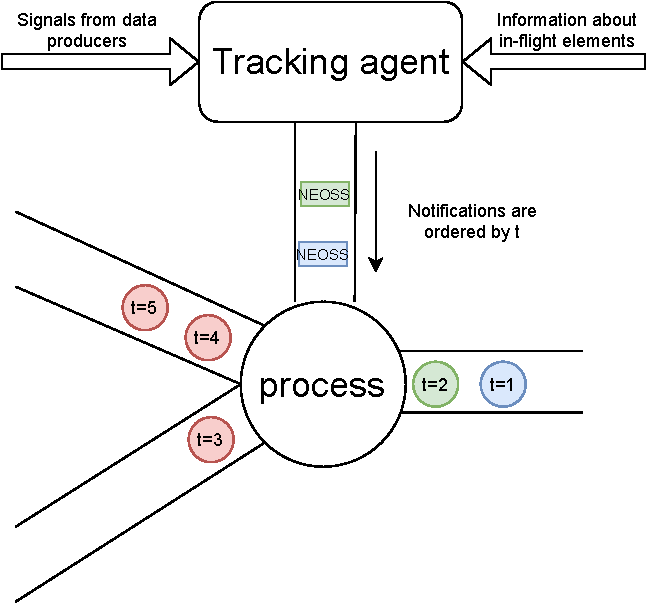
\includegraphics[width=0.30\textwidth]{pics/tracker-ordering.pdf}
  \caption{\tracker\ framework: tracking agent sends NEOSS elements according to the order on t(m)}
  \label{tracker_ordering}
\end{figure}

A vital question here is how to implement the assignment of ordered labels $t(m)$. One way is to use the {\em time oracle} service~\cite{10.14778/3055330.3055335} which can provide totally ordered labels. A simple alternative is discussed in the next section. 

\subsection{Answering Q4: What are the functional and performance properties of \tracker?}
\label{tracker-properties}

\tracker\ does not require regular broadcasting of the elements to all computational nodes because all service traffic goes through a single agent. This change allows \tracker\ to have the following properties by design:

{\bf Cyclic dataflows support.} Because the tracking agent is monitoring the properties of in-flight elements without directly injecting service items into a dataflow, \tracker\ does not have the problem of throwing them through a cycle.

{\bf Low network overhead.} Processes can send reports once per a fixed time period, so there is a constant time of such reports per a finite substream. The reports require $O(|\Pi|)$ extra messages, while the NEOSS events $O(K|\Pi|)$. The total amount is $O(K|\Pi| + |\Pi|) = O(K|\Pi|)$ that is optimal for the substream management problem.

Both of these properties are enhancements over the punctuations framework. They lead to an important corollary: 

{\bf Low latency and impact on SPE throughput.} Punctuations can be stuck by other data elements if they are sent with some delay after the last substream element. In \tracker, service traffic goes through other network channels that can reduce latency between actual substream termination and the corresponding event. Together with the low amount of service traffic, this scheme does not significantly reduce the throughput of an SPE, as we show in Section~\ref{fs-experiments}.

In the next section we theoretically proof the first two properties. The fairness of the corollary is experimentally demonstrated in Section~\ref{fs-experiments}.

% At the same time, \tracker\ can provide both soft and firm bound guarantees along with the consistent order of notifications. A limitation of the \tracker\ framework is a potentially more complex implementation. The details of the straightforward implementation of the \tracker\ framework are discussed in the next section.

\section{Tracker Implementation}
\label {fs-acker-impl}

In the previous section, we introduced a general schema of the \tracker\ framework. In this section, we deepen into its implementation details. We describe and explore the properties of the tracking agent that produces the substream termination notifications (NEOSS). After that, the technique to achieve consistent termination events order is detailed.

\subsection{Bound guarantees}

The tracking agent splits the workflow graph into partially ordered segments and tracks them separately. For each process $p$, we can generate a list of preceding segments that include a set of incoming messages generators $W_p$ for the process. As soon as all these segments contain no elements of a substream, the agent sends to a process {\em NEOSS}.

To track the messages path through segments, the agent receives SND/RCV reports containing a segment identifier and a list of predicates the message satisfies. The agent aggregates this information into the table illustrated in Table~\ref{tracker-table-simple}.

\begin{table}[htbp]
\caption{\tracker\ table: a general example}
  \label{tracker-table-simple}
  \centering
  \footnotesize
  \begin{tabular}{|c|c|c|>{\bfseries}c|} 
    \hline
    Notified & Predicate & Segment & Substream elements  \\ \hline \hline
    \multirow{2}{*}{\checkmark} & \multirow{2}{*}{h(x)} & A & No \\ \cline{3-4}
    & & B & No \\ \hline
    \multirow{2}{*}{} & \multirow{2}{*}{q(x)} & A & No \\ \cline{3-4}
    & & B & Yes \\ \hline
    \multirow{2}{*}{\checkmark} & \multirow{2}{*}{z(x)} & A & No \\ \cline{3-4}
    & & B & No \\ \hline
  \end{tabular}
\end{table}

% A graph shown in Figure~\ref{fig:tracker-acker-comparison} illustrates the notion of segments. This graph has two segments: $A$ and $B$. Note that according to Table~\ref{tracker-table-simple}, the NEOSS for predicate $q(x)$ can be sent for a segment $A$, but not for a segment $B$. This behavior is similar to punctuations: NEOSS can be spawned earlier for the upstream processes.

% \begin{figure}[htbp]
%   \centering
%   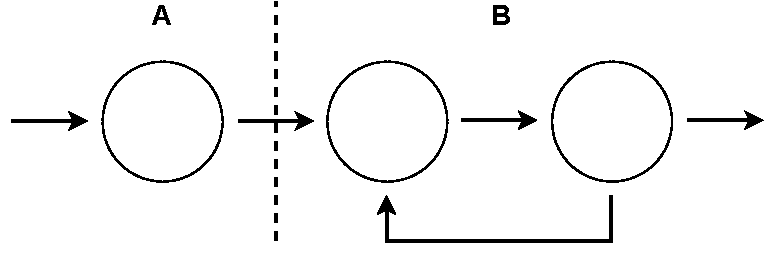
\includegraphics[width=0.3\textwidth]{pics/segments-example.pdf}
%   \caption{Graph segmentation example}
%   \label{fig:tracker-acker-comparison}
% \end{figure}

There are several possible methods to build the indicator that the segment contains elements from a substream using the reports from processes. Our implementation uses the trick applied in Apache Storm to monitor the completeness of processing~\cite{apache:storm:acker}. 

Each report is labeled by a random number $X$, and this number is the same for the send action and the corresponding receive action. This trick makes it easy to check if the segment contains a full set of $SND$/$RCV$ pairs for a message: XOR operation for all numbers received from the chain will turn into 0. The result of the XOR operation can accidentally become zero, but the probability of this event is controlled by the length of the random number $X$ so that it can be neglected in practice~\cite{apache:storm:acker}.

\begin{figure}[t]
  \centering
  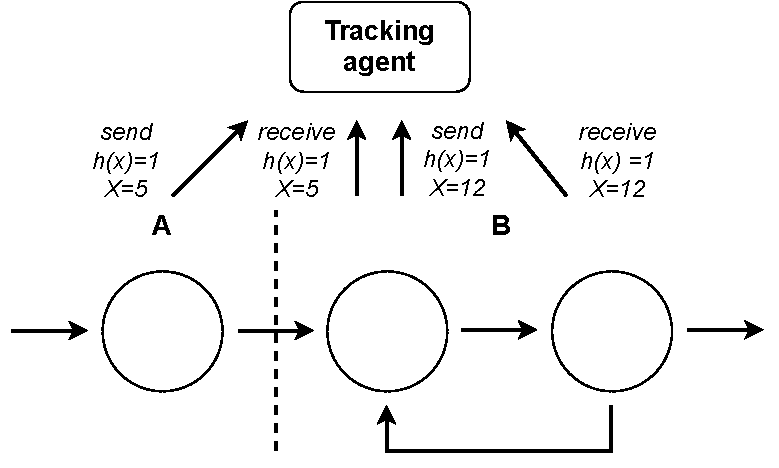
\includegraphics[width=0.25\textwidth]{pics/tracker-segments-example.pdf}
  \caption{Reports example}
  \label{fig:tracker-reports}
\end{figure}

Figure~\ref{fig:tracker-reports} illustrates the reports with random numbers. The elements satisfying a predicate $h(x)$ flow through a dataflow. The first process generates an output and sends the SND report with $X=5$. The corresponding RCV report by the second process also has $X=5$ because this process receives the element from the first one. The second process sends a new element that satisfies $h(x)$ further, and the new SND report with $X=12$ is produced. The third operator receives this element and also produces an RCV report with $X=12$. If there are no more elements such that $h(x)=1$, then we can send NEOSS for the substream defined by $h(x)$ ends because {\em 5 XOR 5 XOR 12 XOR 12 = 0}. Table~\ref{tracker-table-xor} illustrates the actual \tracker\ table for the mentioned technique.

% All reports from processes are grouped by the satisfying predicate and the segment. Random numbers from these reports are XORed into the result shown in columns {\em Segment XOR} and {\em XOR}. If the XOR value is equal to 0, then the tracking agent can send the NEOSS, providing the soft bound guarantee for the corresponding predicate.

\begin{table}[htbp]
\caption{\tracker\ table: XORing technique example}
  \label{tracker-table-xor}
  \centering
  \footnotesize
  \begin{tabular}{|c|c|c|>{\bfseries}c|>{\bfseries}c|} 
    \hline
    Notified & Predicate & Segment & Segment XOR & XOR  \\ \hline \hline
    \multirow{2}{*}{\checkmark} & \multirow{2}{*}{h(x)} & A & 000 & \multirow{2}{*}{000} \\ \cline{3-4}
    & & B & 000 & \\ \hline
    \multirow{2}{*}{} & \multirow{2}{*}{q(x)} & A & 000 & \multirow{2}{*}{110} \\ \cline{4-4}
    & & B & 110 & \\ \hline
    \multirow{2}{*}{\checkmark} & \multirow{2}{*}{z(x)} & A & 000 & \multirow{2}{*}{000} \\ \cline{3-4}
    & & B & 000 & \\ \hline
  \end{tabular}
\end{table}

Due to the associativity of XOR, we can optimize tracking agent incoming traffic by aggregating reports locally within the processes. For each process, we introduce a {\em local tracking agent} component. It serves as a mediator between the process and the global agent, buffering the outgoing reports and flushing them periodically. 

The flushing window is the parameter that allows us to balance the service traffic and latency between the actual substream termination (the event from the data producer) and the termination event. Note that substreams last a finite time period by definition, so we assume that each process sends aggregated reports a constant number of times that does not depend on the number of substreams and processes. Therefore, the amount of extra network traffic for the reports is $O(|\Pi|)$, so the total estimation with the overhead on the notifications is $O(K|\Pi|)$.

\subsection{Consistent termination events order}

If the order of NEOSS is consistent, the order of termination events will be consistent as well. To achieve consistent order of NEOSS, we need to define $t(M)$ such that the order on $t(M)$ respects the order of input elements. All reports that processes send to the tracking agent should be labeled with $t(M)$. In turn, the tracking agent sends the NEOSS elements according to the order on $t(<)$.

Table~\ref{tracker-table-oder} illustrates the \tracker\ table in case of consistent NEOSS order. Column {\em min t(x)} indicates the minimal $t(x)$ among the elements that satisfy the corresponding predicate. The tracking agent sends notifications for the substream if the $XOR$ value is 0 and all substreams that contain elements with less {\em min t(x)} have finished (notifications have been produced). Therefore, NEOSS for the substream defined by the predicate $h(x)$ is not sent until the NEOSS for the predicate $q(x)$ is generated. 

\begin{table}[htbp]
\caption{\tracker\ table: consistent NEOSS order example}
  \label{tracker-table-oder}
  \centering
  \footnotesize
  \begin{tabular}{|c|c|>{\bfseries}c|c|} 
    \hline
    Notified & Predicate & min t(x) &  XOR  \\ \hline \hline
    \multirow{2}{*}{waits for q(x) finish} & \multirow{2}{*}{h(x)} & \multirow{2}{*}{5} & \multirow{2}{*}{000} \\
    & & & \\ \hline
    \multirow{2}{*}{} & \multirow{2}{*}{q(x)} & \multirow{2}{*}{4} & \multirow{2}{*}{110} \\
    & & & \\ \hline
    \multirow{2}{*}{\checkmark} & \multirow{2}{*}{z(x)} & \multirow{2}{*}{1} & \multirow{2}{*}{000} \\
    & & & \\ \hline
  \end{tabular}
\end{table}

If input elements arrive through a single node, $t(x)$ can denote the monotonic system time of the element $x$ arrival. If there are multiple source processes, one can use time oracle agent~\cite{10.14778/3055330.3055335} as a service for generation a monotonic sequence of unique timestamps. However, in this case, there is a need to manage one more subsystem.

A simple technique to build $t(x)$ without extra agents bases on systematic synchronization of the system clocks. We call this method and associated labels {\em coarse time}. Assume that clock differences are no more than some fixed $\delta$, which we reference as synchronization slack. Let $\tau(x)$ be precise physical time of input data item $x$ arrival, and $s(x)$ be local system time of the source node where $x$ arrived. The true order of events $\tau(d_1) > \tau(d_2)$ coming from different sources can be sometimes restored by their system timestamps $s(d_1)$ and $s(d_2)$. If these timestamps differ more than time synchronization slack, then the order is clear: $s(d_1) > s(d_2) + \delta \Rightarrow \tau(d_1) > \tau(d_2)$.

This fact allows us to define $t(x)$ such that $t(x) = [s(x) / \delta]$. This way we make $t(x)$ less precise, but this trick gives us an ability to compare global time associated by different source nodes. If $t(x_1)$ is greater than the $(t(x_2) + 1)$ then their order is defined even if they arrived from different source nodes:  $t(x_1) > t(x_2) + 1 \Rightarrow \tau(x_1) > \tau(x_2)$. Therefore, the order on $t(x)$ coincides with the order of input elements, so it is suitable for the defined problem. Here is a summary of the mechanism that ensures consitent termination events order:
\begin{enumerate}
    \item On input item arrival, source node gets the system timestamp
    \item The system timestamp is shrunk up to synchronization slack (practically we achieve 10ms slack)
    \item Each report for the tracking agent is labeled by the result of $t(x)$
    \item Tracking agent sends NEOSS according to the order on $t(x)$
    \item Termination events are generated according to the order of NEOSS arriving
\end{enumerate}

% \subsection{Distributed tracking agent}

% The tracking agent accumulates all the service traffic from the entire system. To ensure scalability, we introduce a distributed version of the tracking agent.

% A straightforward approach is to partition predicates between the shards of the tracking agent. For example, one shard can handle all reports for the predicate $h(x)$, while the second all reports for the predicate $q(x)$. Note that the network traffic complexity remains the same $O(K|\Pi|)$ because each process sends each report to only a single shard depending on the predicate.

% The main problem regarding this approach is to enforce the consistent NEOSS order. Centralized agent sends NEOSS through the FIFO network channels, so the NEOSS elements for the same processes cannot be reordered. There can be a race between NEOSS from various shards due to asynchronous network channels in the distributed case.

% A simple solution for this issue is on each NEOSS from a shard to wait for NEOSS from all other shards but with greater $t(x)$. For example, if a process receives NEOSS for some predicate with $\min t(x) = 3$, then it needs to wait until receiving NEOSS with $t(x) > 3$ from all other shards to produce the termination event. However, this method can increase the latency between the substream end and the termination event.

% We employ the vector clock algorithm to mitigate latency overhead. Each process either periodically sends its system time to all tracking agent shards. In turn, tracking agents also periodically sends the minimal vector among the in-flight elements. Therefore, if a process receives NEOSS for some predicate with $\min t(x) = 3, vec=[0,4,1]$, then it needs to wait until receiving of vectors component-wise greater than $[0,4,1]$ from all shards to produce the termination event.

% The vector clock introduction increases the service traffic but allows to eliminate bottleneck from the system. The service traffic complexity remains the same, but the $O$ factor increases. In the experimental section, we will study how significant is this increase.


\section {Experiments}
\label {fs-experiments}

% \begin{figure}
% \centering
% \begin{tikzpicture}[%
%   ->, 
%   >=stealth,
%   shorten >=1pt,
%   node distance=1.2cm,
%   thick,
%   every state/.style={%
%   fill=white,
%   draw=black,
%   text=black
%   }   
%   ]
%     \node[draw, circle] (I_1) [draw=none] {};
%     \node[draw, circle] (I_2) [below of=I_1,draw=none] {};
%     \node[draw, circle] (I_dots) [below of=I_2,draw=none] {};
%     \node[draw, circle] (I_3) [below of=I_dots,draw=none] {};

%     \node[draw, circle] (A_1) [right of=I_1] {};
%     \node[draw, circle] (A_2) [below of=A_1] {};
%     \node[draw, circle] (A_dots) [below of=A_2,draw=none] {$\ldots$};
%     \node[draw, circle] (A_3) [below of=A_dots] {};

%     \node[draw, circle] (B_1) [right of=A_1] {};
%     \node[draw, circle] (B_2) [below of=B_1] {};
%     \node[draw, circle] (B_dots) [below of=B_2,draw=none] {$\ldots$};
%     \node[draw, circle] (B_3) [below of=B_dots] {};

%     \node[draw, circle] (Dots_1) [right of=B_1,draw=none] {$\ldots$};
%     \node[draw, circle] (Dots_2) [below of=Dots_1,draw=none] {$\ldots$};
%     \node[draw, circle] (Dots_dots) [below of=Dots_2,draw=none] {$\ldots$};
%     \node[draw, circle] (Dots_3) [below of=Dots_dots,draw=none] {$\ldots$};

%     \node[draw, circle] (Z_1) [right of=Dots_1] {};
%     \node[draw, circle] (Z_2) [below of=Z_1] {};
%     \node[draw, circle] (Z_dots) [below of=Z_2,draw=none] {$\ldots$};
%     \node[draw, circle] (Z_3) [below of=Z_dots] {};

%     \node[draw, circle] (O_1) [right of=Z_1,draw=none] {};
%     \node[draw, circle] (O_2) [below of=O_1,draw=none] {};
%     \node[draw, circle] (O_dots) [below of=O_2,draw=none] {};
%     \node[draw, circle] (O_3) [below of=O_dots,draw=none] {};

%     \path
%           (I_1) edge (A_1)
%           (I_2) edge (A_2)
%           (I_dots) edge (A_dots)
%           (I_3) edge (A_3)
%           (A_1) edge (B_1)
%           (A_1) edge (B_2)
%           (A_1) edge (B_3)
%           (A_2) edge (B_1)
%           (A_2) edge (B_2)
%           (A_2) edge (B_3)
%           (A_3) edge (B_1)
%           (A_3) edge (B_2)
%           (A_3) edge (B_3)
%           (B_1) edge (Dots_1)
%           (B_1) edge (Dots_2)
%           (B_1) edge (Dots_3)
%           (B_2) edge (Dots_1)
%           (B_2) edge (Dots_2)
%           (B_2) edge (Dots_3)
%           (B_3) edge (Dots_1)
%           (B_3) edge (Dots_2)
%           (B_3) edge (Dots_3)
%           (Dots_1) edge (Z_1)
%           (Dots_1) edge (Z_2)
%           (Dots_1) edge (Z_3)
%           (Dots_2) edge (Z_1)
%           (Dots_2) edge (Z_2)
%           (Dots_2) edge (Z_3)
%           (Dots_3) edge (Z_1)
%           (Dots_3) edge (Z_2)
%           (Dots_3) edge (Z_3)
%           (Z_1) edge (O_1)
%           (Z_2) edge (O_2)
%           (Z_dots) edge (O_dots)
%           (Z_3) edge (O_3)
%           ;
%       \draw[-,thick,decorate,decoration={brace,amplitude=5pt,mirror}]
%             ([xshift=-5pt]I_1.center) -- ([xshift=-5pt]I_3.center) node[midway, left=4pt] {Workers};
%       \draw[-,thick,decorate,decoration={brace,amplitude=5pt}]
%             ([xshift=-5pt, yshift=5pt]A_1.center) -- ([xshift=5pt, yshift=5pt]Z_1.center) node[midway, above=5pt] {Operators};
% \end{tikzpicture}
% \caption{Physical execution graph for experiments} 
% \label{physical_graph}
% \end{figure}

The experiments examine the benefits of the proposed substreams management framework and show how it performs within several real-world scenarios compared to the state-of-the-art alternatives.

{\noindent \bf Experimental setup.} To have an ability to compare various techniques within the same streaming engine, we implemented both \tracker\ and punctuation-based methods on the top of an open-source distributed streaming system called \FlameStream. The  \FlameStream\ has similar to state-of-the-art stream processing systems (Flink, Storm, etc.) functionality and use-cases. We did not exploit any system-specific features during the implementation of substream management methods.

We run all experiments on a cluster of 20 virtual machines with a single CPU and 4 GB RAM from one of the biggest cloud providers. Each node runs a \FlameStream\ worker. We deploy \tracker\ on nodes excluded from regular processing: a single one for centralized configuration and two for distributed configuration. 
% If it is not specified, the number of machines used in an experiment is 20, the graph size is 30, and the granularity is 10. 

We divided our evaluation of \tracker\ framework into two parts. Each of these parts encapsulates logically connected experiments that examine the performance of \tracker\ mechanism in various perspectives.

{\noindent \bf Overall performance.} In Section~\ref{overhead}, we demonstrate the performance of the \tracker\ framework itself. First, we measure the amount of extra network traffic for different cluster sizes, the number of nodes in a logical graph, and the sizes of substreams. We also show throughput overhead on regular processing for a fixed streaming setup. Second, we evaluate notifications latency, i.e., the time interval between substream ends and the corresponding notifications are received by subscribers.  Eventually, we demonstrate \tracker\ scalability due to its distributed implementation. 

As a baseline approach, we utilize the punctuations-based method employed in many state-of-the-art stream processing systems such as Flink~\cite{Carbone:2017:SMA:3137765.3137777}, Storm~\cite{apache:storm:state}, Heron~\cite{Kulkarni:2015:THS:2723372.2742788}, IBM Streams~\cite{jacques2016consistent}, etc. To the best of our knowledge, the punctuation framework is the only existing general-purpose substreams management technique.

{\noindent \bf Real-world scenarios.} Section~\ref{real-world-scenarios} contains the evaluation of \tracker\ applied to several real-world problems. The first problem is state garbage collection. Often, the state maintained by streaming operators is divided by keys. When some keys become out-of-date (e.g., data source promises that it will never send elements with such keys further), the corresponding state should be removed. Otherwise, a streaming operator may run out-of-memory. A simple but efficient solution is to apply a fixed-sized LRU cache that spills outdated data on disk. We compare two strategies for freeing keys in the cache:
\begin{enumerate}
    \item Free keys using some pre-defined TTL.
    \item Free keys on notifications by \tracker\ and punctuations that there will be no more elements with such keys.
\end{enumerate}
As a performance metric, we use the cache misses ratio.

The second scenario is hot keys detection. The distribution of keys of data elements that entering SPE can be skewed, and some (hot) keys can occur very often. In this case, load distribution between computational nodes may be imbalanced, and the throughput of an SPE may decrease~\cite{liao2019efficient}. If SPE is able to detect hot keys, it can forbid entering elements with such keys or rebalance load distribution. In this scenario, we evaluate \tracker\ latency and accuracy of hot keys detection. As a baseline approach, we use a naive method that counts keys occurrences independently on each computational node.

The third problem is state snapshotting. Many state-of-the-art stream processing systems, including Flink~\cite{Carbone:2017:SMA:3137765.3137777}, Storm~\cite{Toshniwal:2014:STO:2588555.2595641}, and Samza~\cite{Noghabi:2017:SSS:3137765.3137770}, use state snapshotting protocol~\cite{2015arXiv150608603C} for fault tolerance that requires substreams management. Although this technique is popular, it leads to latency spikes that depend on the latency of notifications that a substream (epoch) ends. In our experiments, we compare latency spikes for punctuations and \tracker\ substreams management frameworks within this state snapshotting protocol.

{\noindent \bf Workloads.} An execution graph for the overall \tracker\ evaluation should be flexible in order to analyze performance with less bias on a specific task. We use synthetic directed graphs of various lengths. All vertices pass an input element to the next operation. All items are re-partitioned (round-robin) before each vertex, as it is shown in Figure~\ref{physical_graph}. This setup does not induce possible overhead by heavy computations while covering many realistic scenarios. Graphs with few vertices (under 30) may fit almost any acyclic streaming pipeline~\cite{akidau2018streaming}. On the other hand, more massive pipelines can be considered as flattened iterative dataflows such as PageRank or Connected Components~\cite{Murray:2013:NTD:2517349.2522738, xu2016efficient}.

For the practical scenarios, we apply two workloads that are representative for todays stream processing problems. The first is breadth-first-search computation on a big social graph. This execution graph can be used for social networks near real-time analysis~\cite{wang2011understanding}. Another application is heuristic search algorithms applied in motion planning for robotics~\cite{sud2007real}. As a dataset for this execution graph, we employ a large social graph provided by Twitter~\cite{kwak2010twitter}. This workload has several distinctive features:
\begin{enumerate}
    \item The execution graph is cyclic. It allows us to evaluate the performance of \tracker\ for cyclic dataflows, where punctuations are inapplicable.
    \item As we demonstrated in Section~\ref{intro-examples}, the state of this dataflow is growing fast, so it can easily run out-of-memory without garbage collection of outdated keys.
    \item Vertices of a social graph are used as keys in this dataflow. Some of them may have significantly more edges than others. Therefore, the load distribution can be imbalanced, and an SPE may require hot keys detection.
\end{enumerate}

The second workflow is near real-time text classification. It has a wide range of applications, including detection of emerging news and current user interests, suspicious traffic analysis, spam filtering, etc~\cite{webirte}. As a dataset, we used an open corpus of news articles from Russian media resource lenta.ru~\cite{lentaru}. This workload has the following properties:
\begin{enumerate}
    \item The state of this dataflow is growing fast as well, so it also requires keys garbage collection.
    \item The dataflow is acyclic so that we can compare \tracker\ with punctuations within garbage collection and state snapshotting tasks.
    \item This dataflow uses TF-IDF as a feature for text classification. Words are used as keys to compute IDF. Hence, the load distribution can be imbalanced due to Zipf law. This scenario may also require hot keys detection in order to rebalance load more optimal. 
\end{enumerate}

% We measure the notification latency within various setups as well as the ability of distributed \tracker\ to scale out. Finally, in section~\ref{snapshotting}, we analyze the performance of operator-level tracking with the state snapshotting problem. 

% As a baseline approach, we utilize the marker-based method employed in many state-of-the-art stream processing systems such as Flink~\cite{Carbone:2017:SMA:3137765.3137777}, Storm~\cite{apache:storm:state}, Heron~\cite{Kulkarni:2015:THS:2723372.2742788}, IBM Streams~\cite{jacques2016consistent}, etc. This technique, as well as alternatives, is detailed in Section~\ref{existing_solutions}. Unlike other mentioned techniques, markers support fine granularity and operator-level locality of tracking. 

% To have an ability to compare two techniques within the same streaming engine, we implemented both \tracker\ and marker methods on the top open-source distributed streaming system called \FlameStream. The  \FlameStream\ has similar to state-of-the-art stream processing systems (Flink, Storm, etc.) functionality and use-cases. We did not exploit any system-specific features during the implementation of tracking methods.

% We decided to compare the approaches within the same stream processing engine to neglect possible performance differences in serialization, settings, platform-specific optimizations, etc. Our goal is to compare the asymptotically better (in terms of network traffic overhead) solution with less theoretically performant one within a practical problem.

% As a logical graph for experiments, we use simple directed graphs of various lengths. All vertices pass an input element to the next operation. All items are re-partitioned (round-robin) before each vertex, as it is shown in Figure~\ref{physical_graph}. This setup does not induce possible overhead by heavy computations while covering many real-life scenarios. Graphs with few vertices (under 30) may fit almost any acyclic streaming pipeline~\cite{akidau2018streaming}. On the other hand, more massive pipelines can be considered as flattened iterative dataflows such as PageRank or Connected Components~\cite{Murray:2013:NTD:2517349.2522738, xu2016efficient}.

% We run all experiments on a cluster of 20 virtual machines with a single CPU and 4 GB RAM from one of the biggest cloud providers. Each node runs a \FlameStream\ worker. We deploy \tracker\ on nodes excluded from regular processing: a single one for centralized configuration and two for distributed configuration. If it is not specified, the number of machines used in an experiment is 20, the graph size is 30, and the granularity is 10. 

\subsection{\tracker\ performance} \label{overhead}

\subsubsection{Network traffic}

\subsubsection{Overhead on SPE throughput}

\subsubsection{Notification latency}

\subsubsection{Scalability}

\subsection{Real-world scenarios} \label{real-world-scenarios}

\subsubsection{State garbage collection}

\subsubsection{State snapshotting}

\subsubsection{Hot keys detection}

% \begin{figure}
% \centering
% \begin{tikzpicture}[%
%   ->, 
%   >=stealth,
%   shorten >=1pt,
%   node distance=1.2cm,
%   thick,
%   every state/.style={%
%   fill=white,
%   draw=black,
%   text=black
%   }   
%   ]
%     \node[draw, circle] (I_1) [draw=none] {};
%     \node[draw, circle] (I_2) [below of=I_1,draw=none] {};
%     \node[draw, circle] (I_dots) [below of=I_2,draw=none] {};
%     \node[draw, circle] (I_3) [below of=I_dots,draw=none] {};

%     \node[draw, circle] (A_1) [right of=I_1] {};
%     \node[draw, circle] (A_2) [below of=A_1] {};
%     \node[draw, circle] (A_dots) [below of=A_2,draw=none] {$\ldots$};
%     \node[draw, circle] (A_3) [below of=A_dots] {};

%     \node[draw, circle] (B_1) [right of=A_1] {};
%     \node[draw, circle] (B_2) [below of=B_1] {};
%     \node[draw, circle] (B_dots) [below of=B_2,draw=none] {$\ldots$};
%     \node[draw, circle] (B_3) [below of=B_dots] {};

%     \node[draw, circle] (Dots_1) [right of=B_1,draw=none] {$\ldots$};
%     \node[draw, circle] (Dots_2) [below of=Dots_1,draw=none] {$\ldots$};
%     \node[draw, circle] (Dots_dots) [below of=Dots_2,draw=none] {$\ldots$};
%     \node[draw, circle] (Dots_3) [below of=Dots_dots,draw=none] {$\ldots$};

%     \node[draw, circle] (Z_1) [right of=Dots_1] {};
%     \node[draw, circle] (Z_2) [below of=Z_1] {};
%     \node[draw, circle] (Z_dots) [below of=Z_2,draw=none] {$\ldots$};
%     \node[draw, circle] (Z_3) [below of=Z_dots] {};

%     \node[draw, circle] (O_1) [right of=Z_1,draw=none] {};
%     \node[draw, circle] (O_2) [below of=O_1,draw=none] {};
%     \node[draw, circle] (O_dots) [below of=O_2,draw=none] {};
%     \node[draw, circle] (O_3) [below of=O_dots,draw=none] {};

%     \path
%           (I_1) edge (A_1)
%           (I_2) edge (A_2)
%           (I_dots) edge (A_dots)
%           (I_3) edge (A_3)
%           (A_1) edge (B_1)
%           (A_1) edge (B_2)
%           (A_1) edge (B_3)
%           (A_2) edge (B_1)
%           (A_2) edge (B_2)
%           (A_2) edge (B_3)
%           (A_3) edge (B_1)
%           (A_3) edge (B_2)
%           (A_3) edge (B_3)
%           (B_1) edge (Dots_1)
%           (B_1) edge (Dots_2)
%           (B_1) edge (Dots_3)
%           (B_2) edge (Dots_1)
%           (B_2) edge (Dots_2)
%           (B_2) edge (Dots_3)
%           (B_3) edge (Dots_1)
%           (B_3) edge (Dots_2)
%           (B_3) edge (Dots_3)
%           (Dots_1) edge (Z_1)
%           (Dots_1) edge (Z_2)
%           (Dots_1) edge (Z_3)
%           (Dots_2) edge (Z_1)
%           (Dots_2) edge (Z_2)
%           (Dots_2) edge (Z_3)
%           (Dots_3) edge (Z_1)
%           (Dots_3) edge (Z_2)
%           (Dots_3) edge (Z_3)
%           (Z_1) edge (O_1)
%           (Z_2) edge (O_2)
%           (Z_dots) edge (O_dots)
%           (Z_3) edge (O_3)
%           ;
%       \draw[-,thick,decorate,decoration={brace,amplitude=5pt,mirror}]
%             ([xshift=-5pt]I_1.center) -- ([xshift=-5pt]I_3.center) node[midway, left=4pt] {Workers};
%       \draw[-,thick,decorate,decoration={brace,amplitude=5pt}]
%             ([xshift=-5pt, yshift=5pt]A_1.center) -- ([xshift=5pt, yshift=5pt]Z_1.center) node[midway, above=5pt] {Operators};
% \end{tikzpicture}
% \caption{Physical execution graph for experiments} 
% \label{physical_graph}
% \end{figure}

% % https://gist.github.com/faucct/032aaf6240db361d30a184b1d7bf3c8e
% \begin{figure*}[t!]
%     \begin{subfigure}[b]{0.32\textwidth}
%             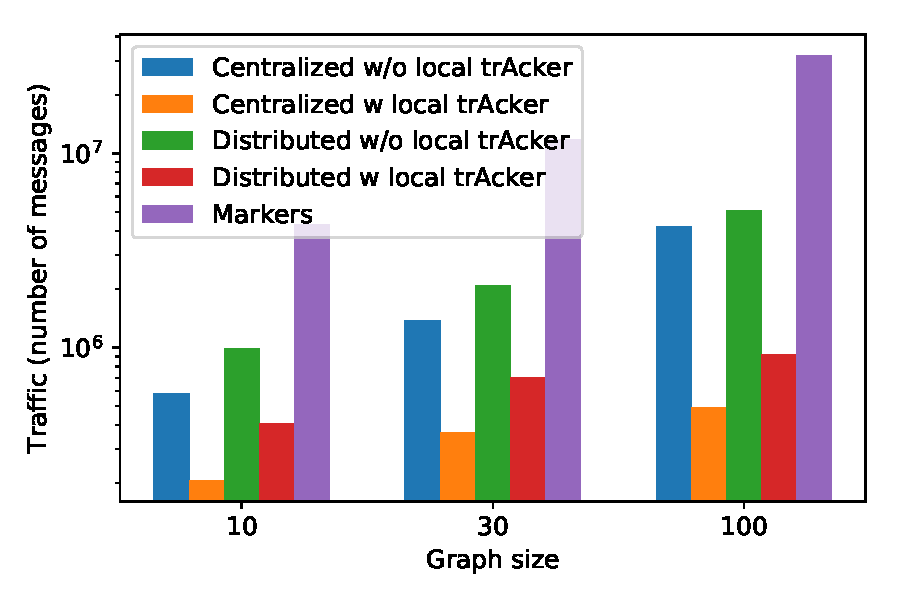
\includegraphics[width=0.99\textwidth]{pics/traffic_by_graph_size_bars.pdf}
%             \caption{Traffic by graph size}
%             \label{traffic_graph}
%     \end{subfigure}
%     \hspace{5mm}
%     \begin{subfigure}[b]{0.32\textwidth}
%             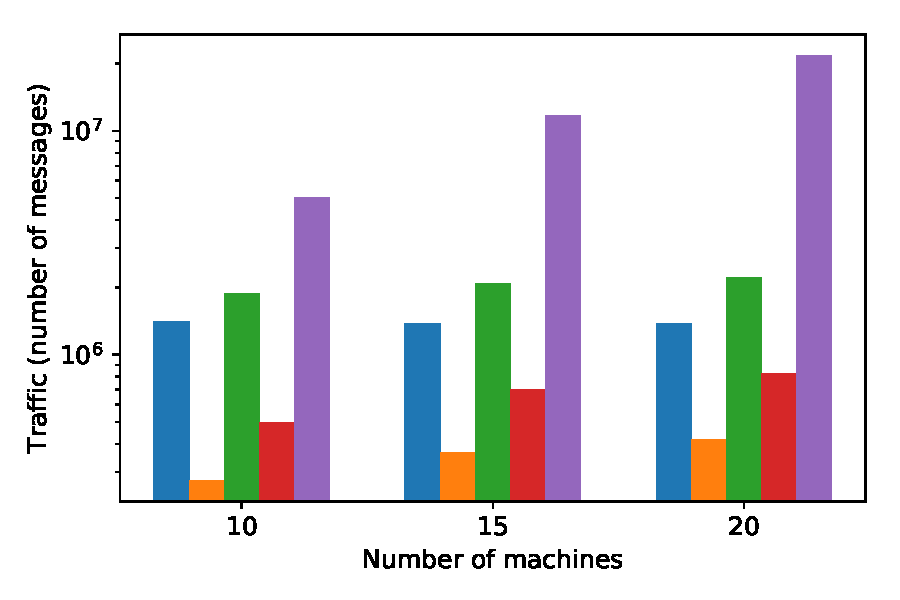
\includegraphics[width=0.99\textwidth]{pics/traffic_by_number_of_machines_bars.pdf}
%             \caption{Traffic by number of virtual machines}
%             \label{traffic_machines}
%     \end{subfigure}
%     \hspace{5mm}
%     \begin{subfigure}[b]{0.32\textwidth}
%             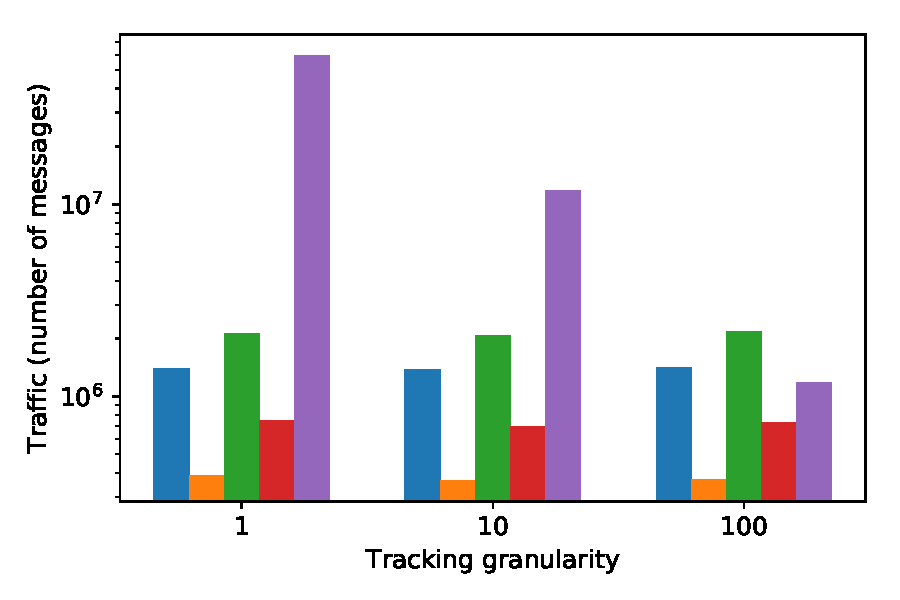
\includegraphics[width=0.99\textwidth]{pics/traffic_by_tracking_frequency_bars.pdf}
%             \caption{Traffic by tracking frequency}
%             \label{traffic_granularity}
%     \end{subfigure}
%     \caption{Service network traffic of marker-based approach and various \tracker\ setups}
%     \label{traffic_plots}
% \end{figure*}

% \label {fs-acker-experiments}

% We divided our evaluation of \tracker\ into three parts. Each of these parts encapsulates logically connected experiments that measure the performance of \tracker\ mechanism in various perspectives.

% In Section~\ref{overhead}, we demonstrate the overhead induced by \tracker\ mechanism. First, we measure the amount of extra network traffic for different cluster sizes, the number of nodes in a logical graph, and the granularity of tracking. After that, we show throughput overhead on regular processing for a fixed streaming setup. Section~\ref{completeness} contains the evaluation of \tracker\ applied to completeness monitoring problem. We measure the notification latency within various setups as well as the ability of distributed \tracker\ to scale out. Finally, in section~\ref{snapshotting}, we analyze the performance of operator-level tracking with the state snapshotting problem. 

% As a baseline approach, we utilize the marker-based method employed in many state-of-the-art stream processing systems such as Flink~\cite{Carbone:2017:SMA:3137765.3137777}, Storm~\cite{apache:storm:state}, Heron~\cite{Kulkarni:2015:THS:2723372.2742788}, IBM Streams~\cite{jacques2016consistent}, etc. This technique, as well as alternatives, is detailed in Section~\ref{existing_solutions}. Unlike other mentioned techniques, markers support fine granularity and operator-level locality of tracking. 

% To have an ability to compare two techniques within the same streaming engine, we implemented both \tracker\ and marker methods on the top open-source distributed streaming system called \FlameStream. The  \FlameStream\ has similar to state-of-the-art stream processing systems (Flink, Storm, etc.) functionality and use-cases. We did not exploit any system-specific features during the implementation of tracking methods.

% We decided to compare the approaches within the same stream processing engine to neglect possible performance differences in serialization, settings, platform-specific optimizations, etc. Our goal is to compare the asymptotically better (in terms of network traffic overhead) solution with less theoretically performant one within a practical problem.

% As a logical graph for experiments, we use simple directed graphs of various lengths. All vertices pass an input element to the next operation. All items are re-partitioned (round-robin) before each vertex, as it is shown in Figure~\ref{physical_graph}. This setup does not induce possible overhead by heavy computations while covering many real-life scenarios. Graphs with few vertices (under 30) may fit almost any acyclic streaming pipeline~\cite{akidau2018streaming}. On the other hand, more massive pipelines can be considered as flattened iterative dataflows such as PageRank or Connected Components~\cite{Murray:2013:NTD:2517349.2522738, xu2016efficient}.

% We run all experiments on a cluster of 20 virtual machines with a single CPU and 4 GB RAM from one of the biggest cloud providers. Each node runs a \FlameStream\ worker. We deploy \tracker\ on nodes excluded from regular processing: a single one for centralized configuration and two for distributed configuration. If it is not specified, the number of machines used in an experiment is 20, the graph size is 30, and the granularity is 10. 

% \subsection{Network usage and overhead} \label{overhead}

% In this section, we demonstrate the overhead that can be induced by \tracker\ and markers techniques. In Section~\ref{exp_network_traffic}, we compare the number of service messages needed for both methods. In Section~\ref{overhead_throughput}, we demonstrate how dependency tracking methods may influence the throughput of a regular stream processing task.

% \subsubsection{Network traffic}
% \label{exp_network_traffic}

% We can measure the extra load provided by tracking mechanisms in a number of service messages sent over the network. In \tracker\ there are several types of these messages: {\em Acks}, {\em Hearbeats}, {\em Min Time Updates}, and {\em Node Times} in distributed setup. In the baseline approach, all service messages are markers. Figure~\ref{traffic_plots} demonstrates the dependency between service network messages and the size of the logical graph, the number of computational nodes, and the granularity of tracking. The extra service traffic is generated by $50K$ input elements sent with 100 items per second arrival rate. 

% As it is shown in Figure~\ref{traffic_graph}, service traffic for markers linearly depends on the dataflow size, because each new logical vertex adds network broadcasting of markers on a physical level. Dependency from the number of computational nodes is quadratic \footnote{At first glance, the dependency may seem linear, but please note that the X-axis covers range from 10 to 20, and the Y-axis is log-scaled} due to the need to broadcast markers to each node after all operators, as it is demonstrated in Figure~\ref{traffic_machines}. Figure~\ref{traffic_granularity} indicates that the number of sent service messages for markers also directly depends on the tracking granularity. For example, the system should broadcast markers after each streaming element in every operator to implement tracking of individual items. 

% In the case of \tracker , service traffic depends on the logical graph size and the number of machines as well. The growth has a linear trend but can be significantly reduced with the local \tracker\ optimization. Distributed \tracker\ without optimizations provides ~10x less service than markers traffic for a graph with 10 vertices, and ~30x decrease for a graph with 100 vertices. Regarding the number of machines, the difference is ~10x for 10 nodes, and ~30x for 20 nodes. Besides, local \tracker\ optimization allows the system to reduce traffic in up to 5 times in comparison with plain distributed \tracker .

% \subsubsection{Overhead on throughput}
% \label{overhead_throughput}

% In this experiment, we measure the median latency of regular processing, depending on the input rate (input elements per millisecond). The growth of median latency indicates system overloading. Input rate that corresponds to the point where latency starts to grow indicates a {\em sustainable throughput}~\cite{karimov2018benchmarking}.

% Figure~\ref{throughput_overhead} demonstrates the results of the experiment. The system without tracking at all starts to be overloaded since $\sim 9K$ requests (items) per second input rate. The system with the finest-grained centralized \tracker\ setup provides $\sim 7K$ RPS sustainable throughput. Overloading with the marker-based approach depends on the granularity of tracking: the finest-grained setup does not sustain even $1K$ RPS, while the setup with the granularity of 10 has $\sim 2K$ RPS throughput. Markers achieve similar to centralized \tracker\ throughput ($\sim 5K$ RPS) only when they are injected once per 50 input elements.

% This experiment shows that markers significantly bound throughput of regular processing within the fine-grained setups. It is explained by the heavy extra network traffic that we demonstrated in the previous experiment. Note that this additional traffic goes through the same network channels as ordinary data items to ensure that markers do not overtake ordinary records. On the other hand, \tracker\ provides less additional system load due to lower extra network usage and the exploiting of additional network channels.

% \begin{figure}[htbp]
%   \centering
%   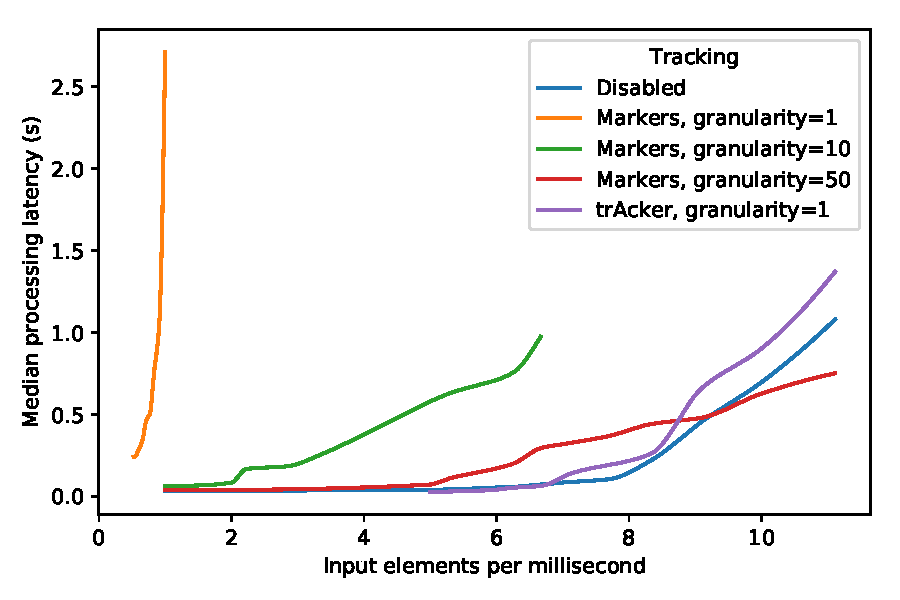
\includegraphics[width=0.50\textwidth]{pics/throughput_overhead_50.pdf}
%   \caption{Tracking overhead on a processing throughput}
%   \label{throughput_overhead}
% \end{figure}

% % https://gist.github.com/faucct/032aaf6240db361d30a184b1d7bf3c8e
% \begin{figure*}[t!]
%     \begin{subfigure}[b]{0.32\textwidth}
%             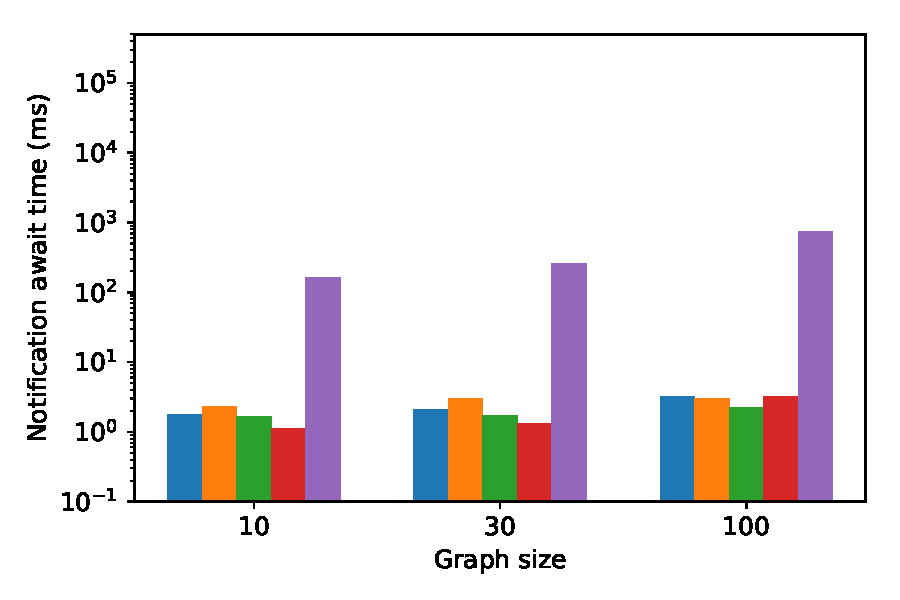
\includegraphics[width=0.99\textwidth]{pics/notification_await_time_by_graph_size_bars.pdf}
%             \caption{Notification latency by graph size}
%             \label{notification_graph}
%     \end{subfigure}
%     \hspace{5mm}
%     \begin{subfigure}[b]{0.32\textwidth}
%             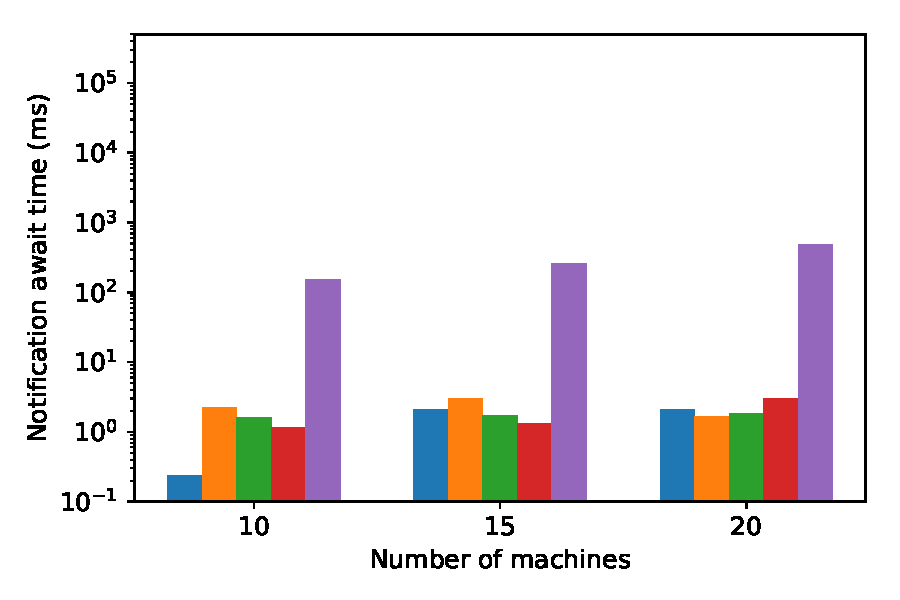
\includegraphics[width=0.99\textwidth]{pics/notification_await_time_by_number_of_machines_bars.pdf}
%             \caption{Notification latency by VMs number}
%             \label{notification_machines}
%     \end{subfigure}
%     \hspace{5mm}
%     \begin{subfigure}[b]{0.32\textwidth}
%             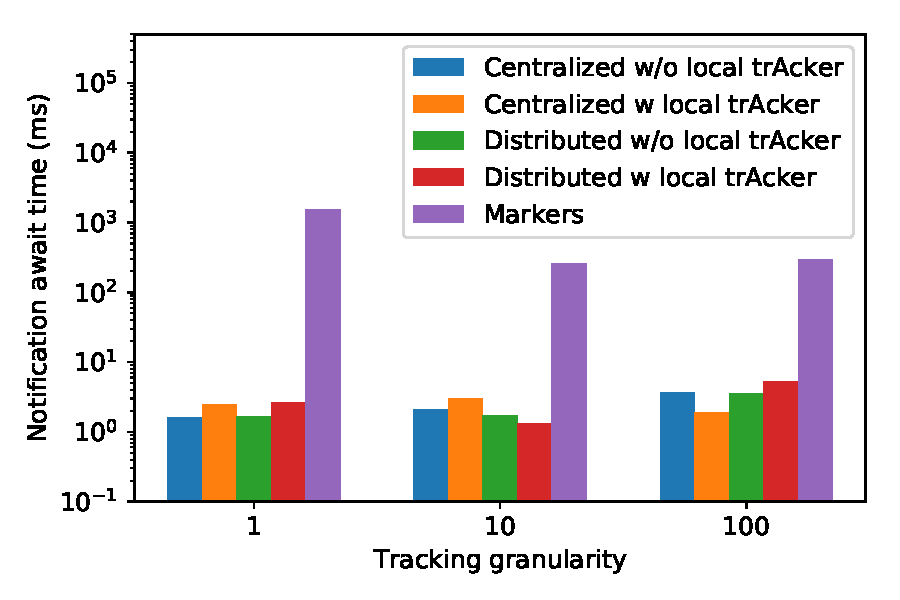
\includegraphics[width=0.99\textwidth]{pics/notification_await_time_by_tracking_frequency_bars.pdf}
%             \caption{Notification latency by granularity}
%             \label{notification_granularity}
%     \end{subfigure}
%     \caption{Notification latency}
%     \label{notification_latency}
% \end{figure*}

% % https://gist.github.com/faucct/546f5617b958349a125449926373b780
% \begin{figure*}[t!]
%     \begin{subfigure}[b]{0.32\textwidth}
%             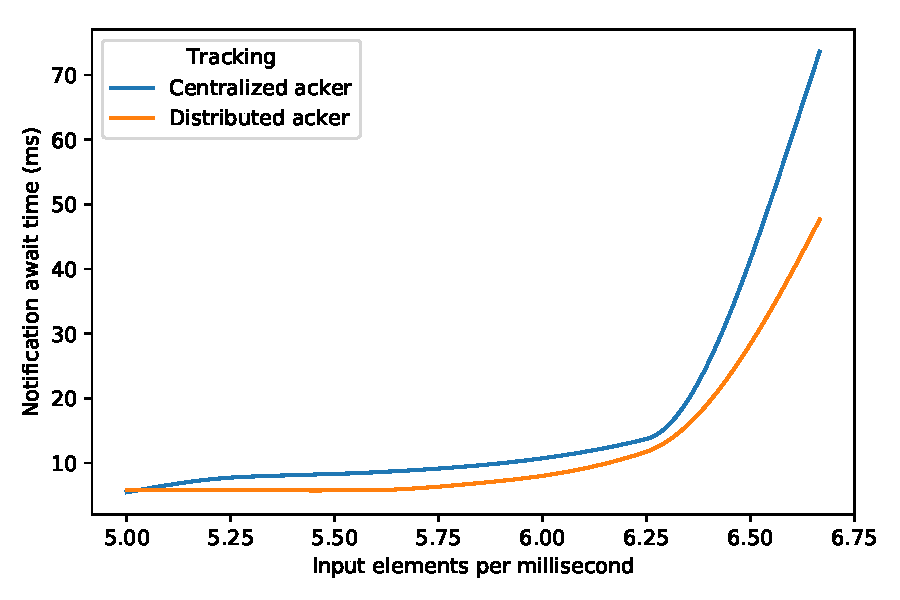
\includegraphics[width=0.99\textwidth]{pics/scalability_01x.pdf}
%             \caption{1x acks}
%             \label{1x_acks}
%     \end{subfigure}
%     \hspace{5mm}
%     \begin{subfigure}[b]{0.32\textwidth}
%             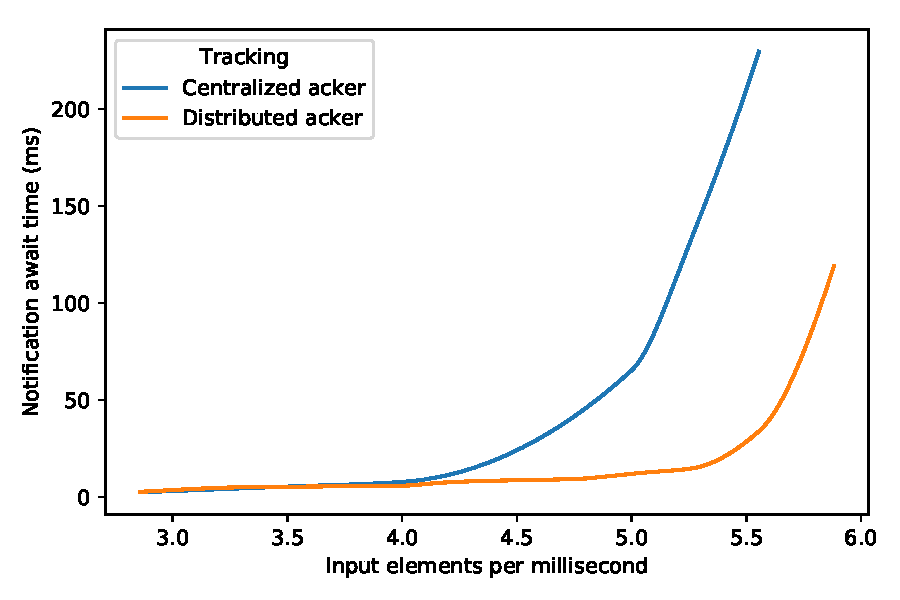
\includegraphics[width=0.99\textwidth]{pics/scalability_05x.pdf}
%             \caption{5x acks}
%             \label{5x_acks}
%     \end{subfigure}
%     \hspace{5mm}
%     \begin{subfigure}[b]{0.32\textwidth}
%             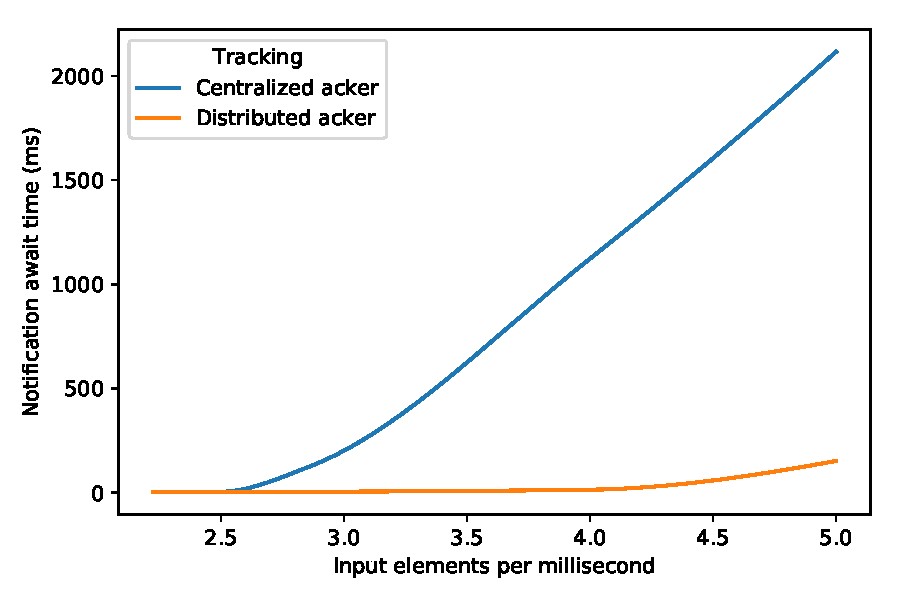
\includegraphics[width=0.99\textwidth]{pics/scalability_09x.pdf}
%             \caption{9x acks}
%             \label{9x_acks}
%     \end{subfigure}
%     \caption{\tracker\ scalability}
%     \label{notification_scalability}
% \end{figure*}

% \subsection{Completeness monitoring} \label{completeness}

% \subsubsection{Notification latency}

% One of the key performance metrics in completeness monitoring solution is the latency of notifications. In some applications~\cite{Carbone:2017:SMA:3137765.3137777, we2018adbis} notification latency directly influences the latency of regular processing. For example, Flink finishes its state snapshotting protocol for the epoch (set of input elements) and delivers corresponding output elements to data consumers only after receiving a notification that the whole epoch is completed. 

% In this experiment, we measure the notification latency as an interval duration between a time moment when a set of input elements has been entirely processed and the reception of the notification for this event. We investigate the dependency between the notification latency and cluster sizes, the number of nodes in a logical graph, and the granularity of tracking. Figure~\ref{notification_latency} shows the results of the experiment. 

% The notification latency of marker-based technique depends on the graph and cluster sizes and the granularity of tracking as figures~\ref{notification_graph},\ref{notification_machines}, and~\ref{notification_granularity} indicate. These results are in-line with the overhead induced by markers shown in Section~\ref{overhead}. Notification latency of \tracker\ slightly fluctuates but does not directly depend on the investigated parameters. One can also note that local \tracker\ optimization, as well as distributed version, do not induce heavy overhead on the latency.

% Such a significant difference in latency between the markers and \tracker\ is explained by the fact that each operator in a dataflow must wait for markers from all partitions of the previous operator to send it further. This behavior ensures that markers do not overtake ordinary records that guarantee the correctness of this approach.

% \subsubsection{Scalability}

% In this experiment, we demonstrate that the distributed version of \tracker\ allows the completeness monitoring mechanism to scale. We measure the median notification latency, depending on the rate of input records. The growth of median latency indicates \tracker\ overloading. Input rate that corresponds to the point where latency starts to grow indicates a {\em sustainable throughput} of the \tracker . To simulate an additional load on the \tracker , staying on a budget of 20 machines, we artificially increased the number of sent service messages in 5 and 9 times. We approximate the sustainable throughput by multiplying extra service messages ratio by the obtained throughput due to the direct dependency between the input and service messages rates. This trick allows us to estimate \tracker\ throughput in a number of input data items per second rate without overloading of the stream processing system itself. Figure~\ref{notification_scalability} demonstrates the results of this experiment.

% Without the extra load, distributed \tracker\ provides similar results as a centralized setup, as Figure~\ref{1x_acks} indicates. Note, overloading of the streaming system limits the throughput of \tracker\ as well because it starts to delay service messages sending, buffer MinTimeUpdates, etc. Figure~\ref{5x_acks} demonstrates that with 5x simulated extra load, distributed \tracker\ can sustain $\sim 27K$ requests (items) per second input rate, while centralized provides only $\sim 20K$ RPS throughput. Figure~\ref{9x_acks} shows that with the increase of the extra load to 9x, distributed \tracker\ provides almost 2x throughput increase: $\sim 40K$ RPS against $\sim 22K$ RPS. 

% The experiments demonstrate that even centralized \tracker\ can sustain a high input rate within 20 computational nodes. Besides, the distributed version of \tracker\ can make the completeness monitoring mechanism scalable in larger setups.

% \begin{figure*}[t!]
%     \begin{subfigure}[b]{0.32\textwidth}
%             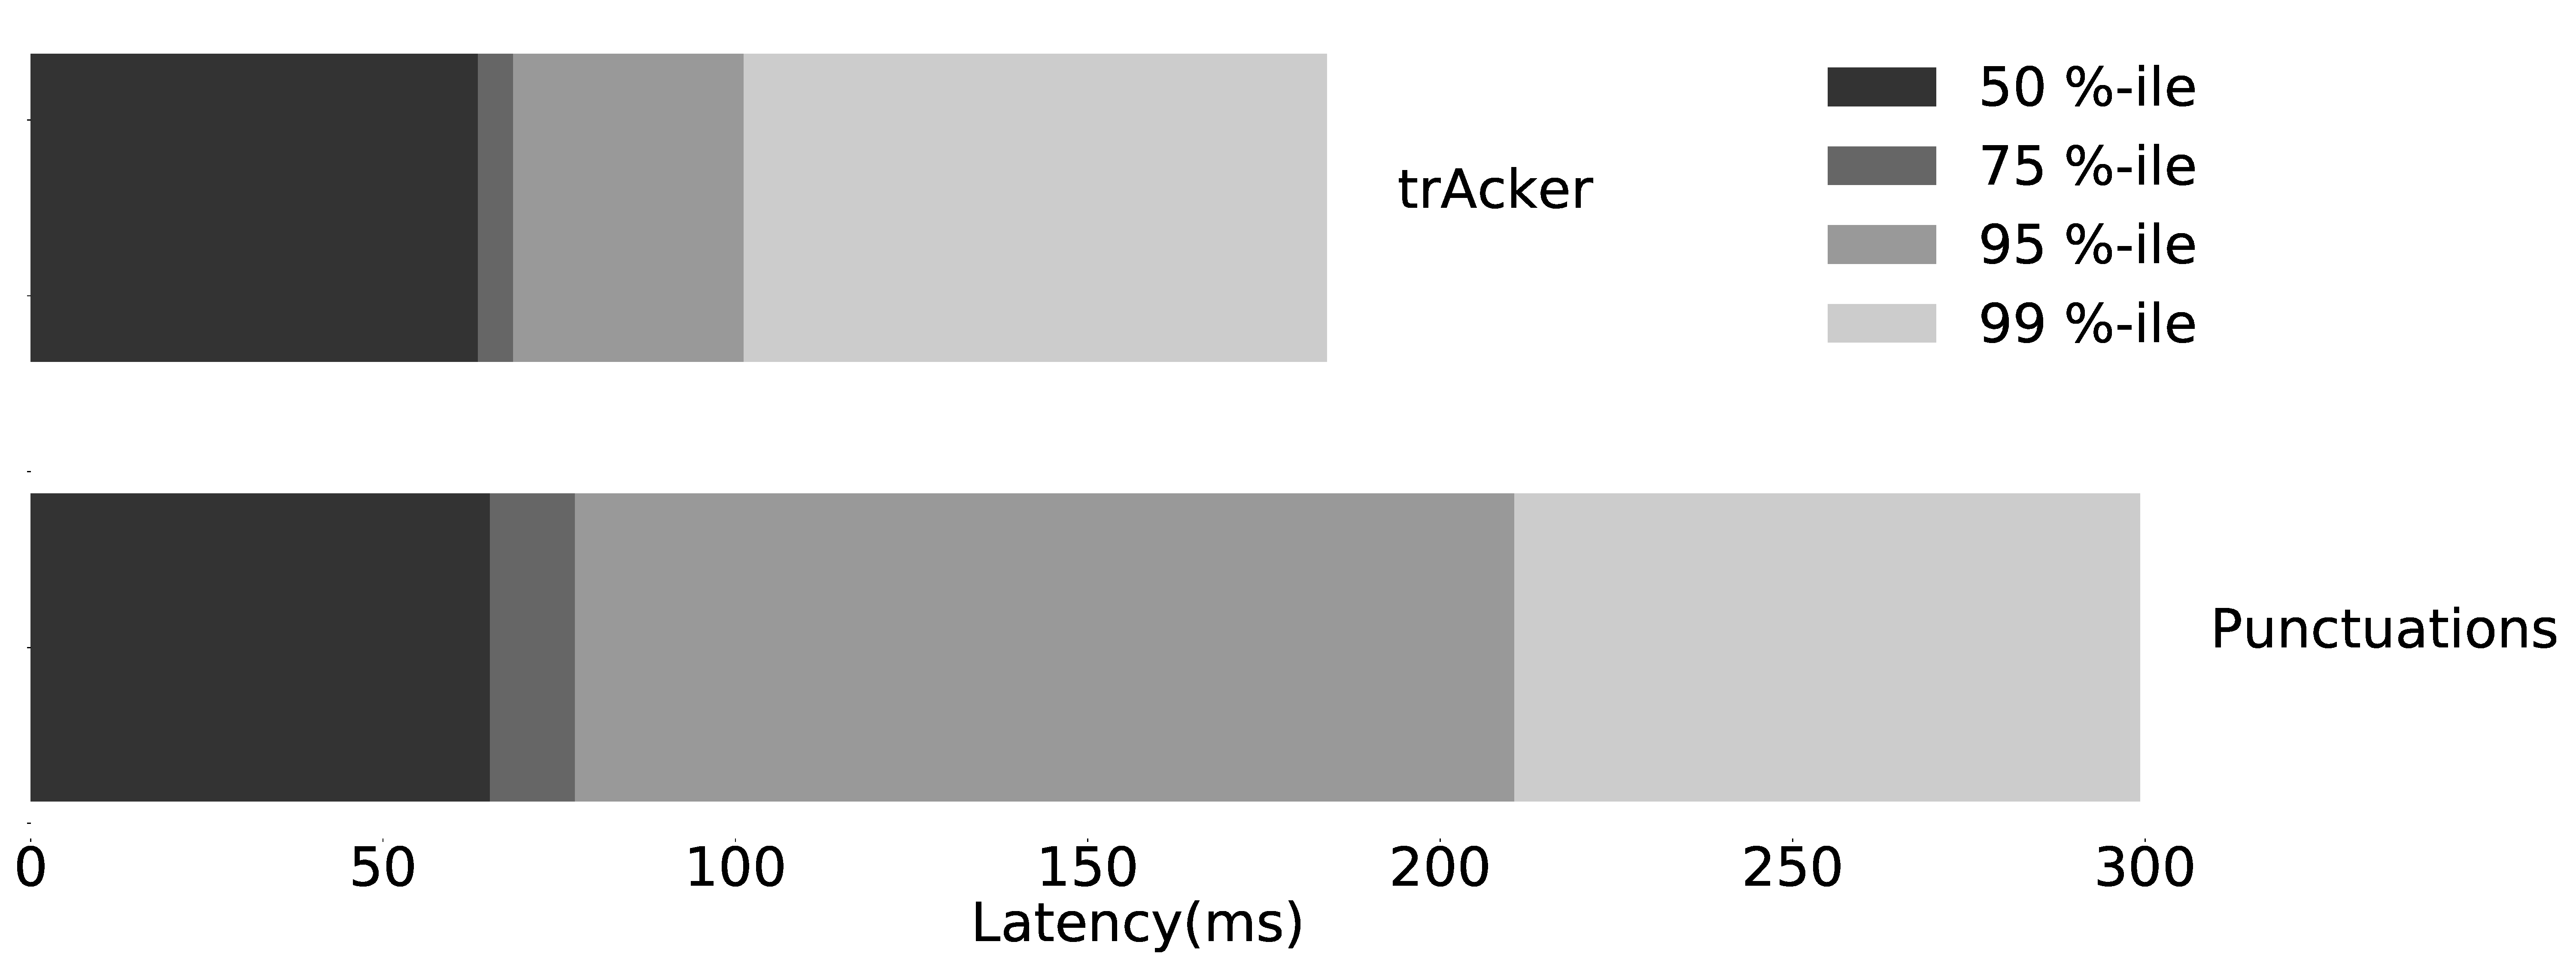
\includegraphics[width=0.99\textwidth]{pics/buffering_latencies_barh_100.pdf}
%             \caption{100 ms snapshot duration}
%             \label{100ms_snapshot}
%     \end{subfigure}
%     \hspace{5mm}
%     \begin{subfigure}[b]{0.32\textwidth}
%             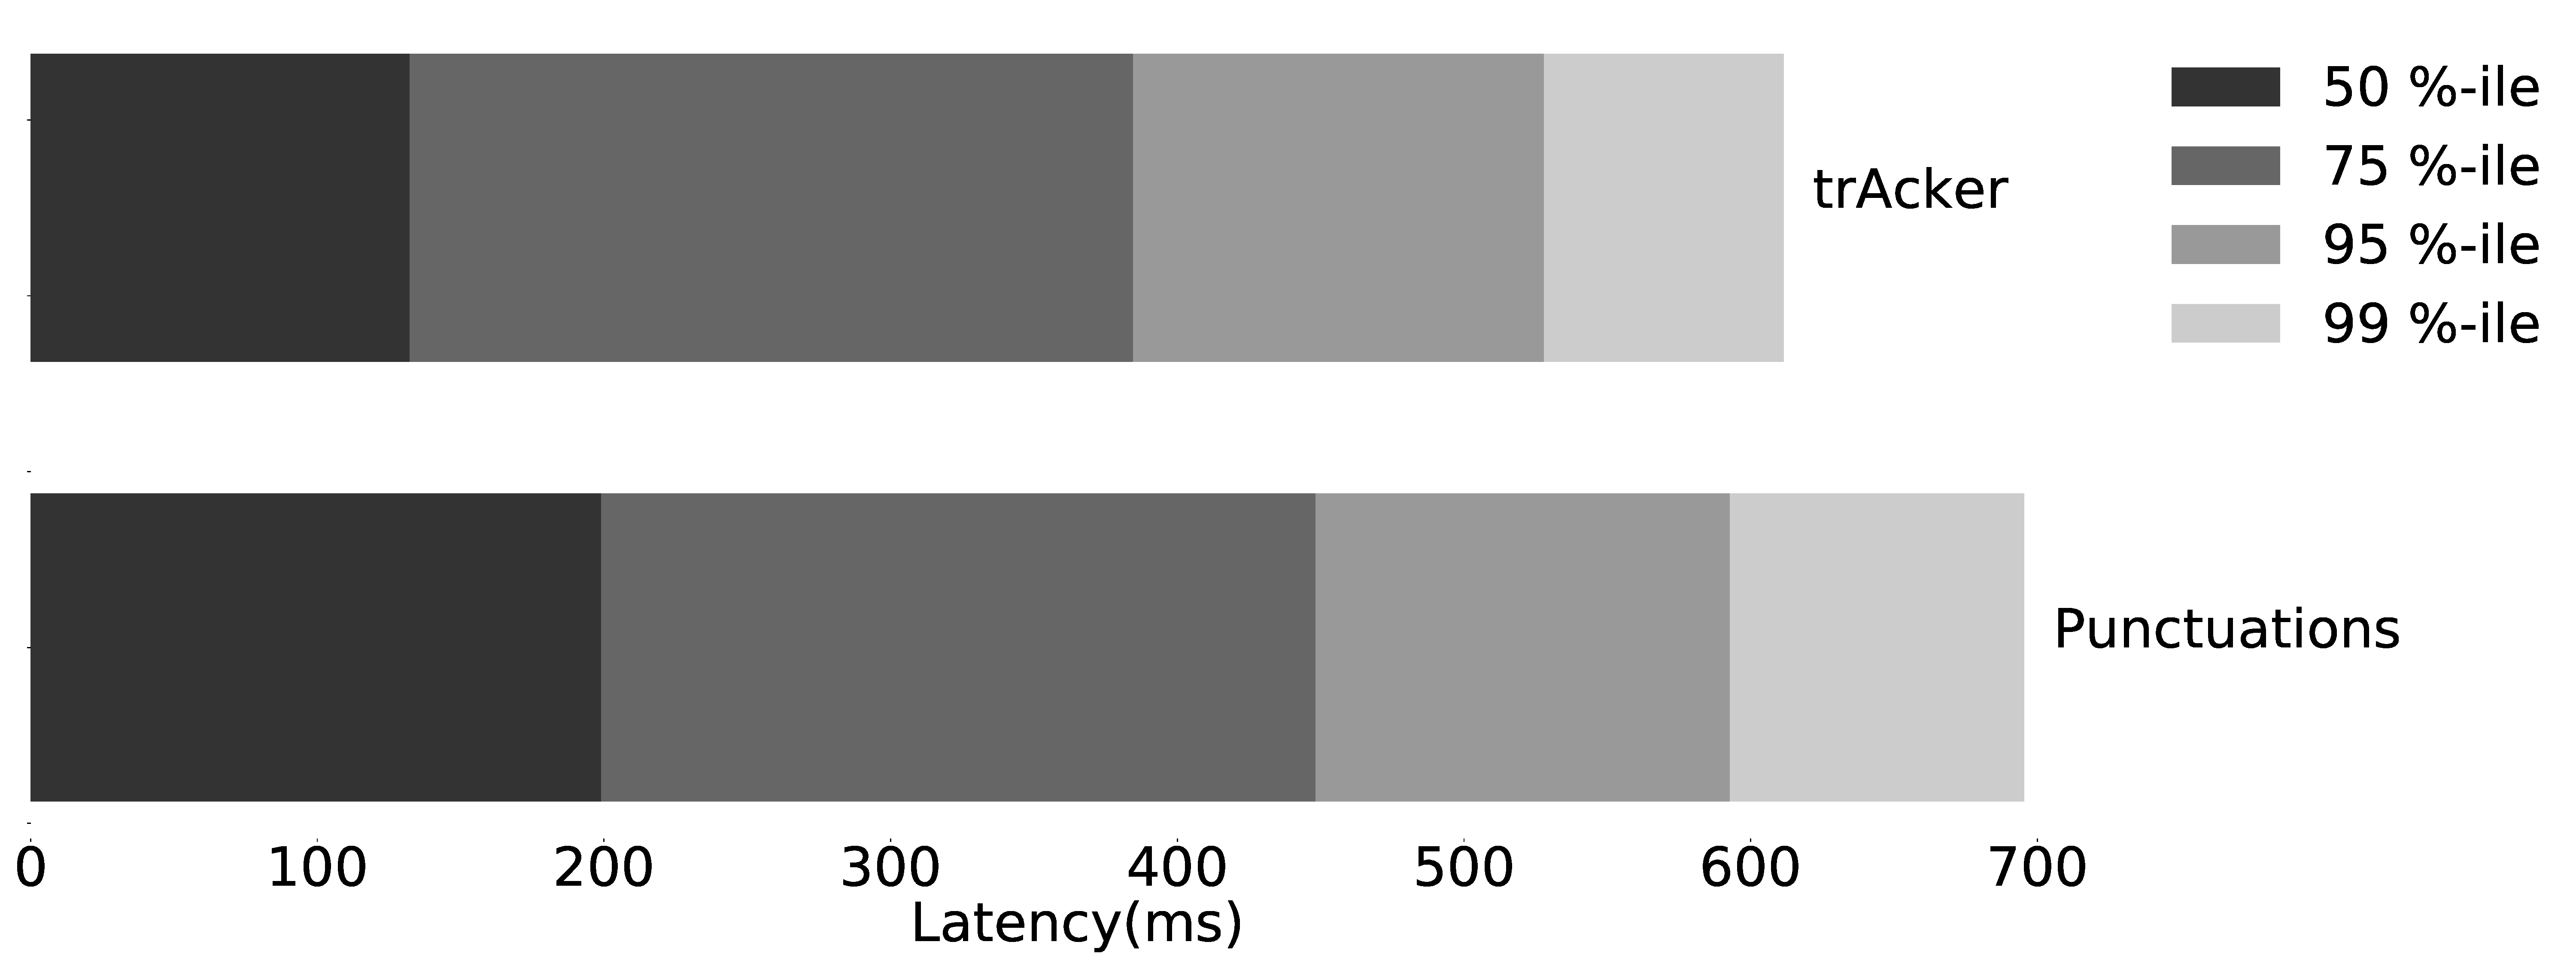
\includegraphics[width=0.99\textwidth]{pics/buffering_latencies_barh_500.pdf}
%             \caption{500 ms snapshot duration}
%             \label{500ms_snapshot}
%     \end{subfigure}
%     \hspace{5mm}
%     \begin{subfigure}[b]{0.32\textwidth}
%             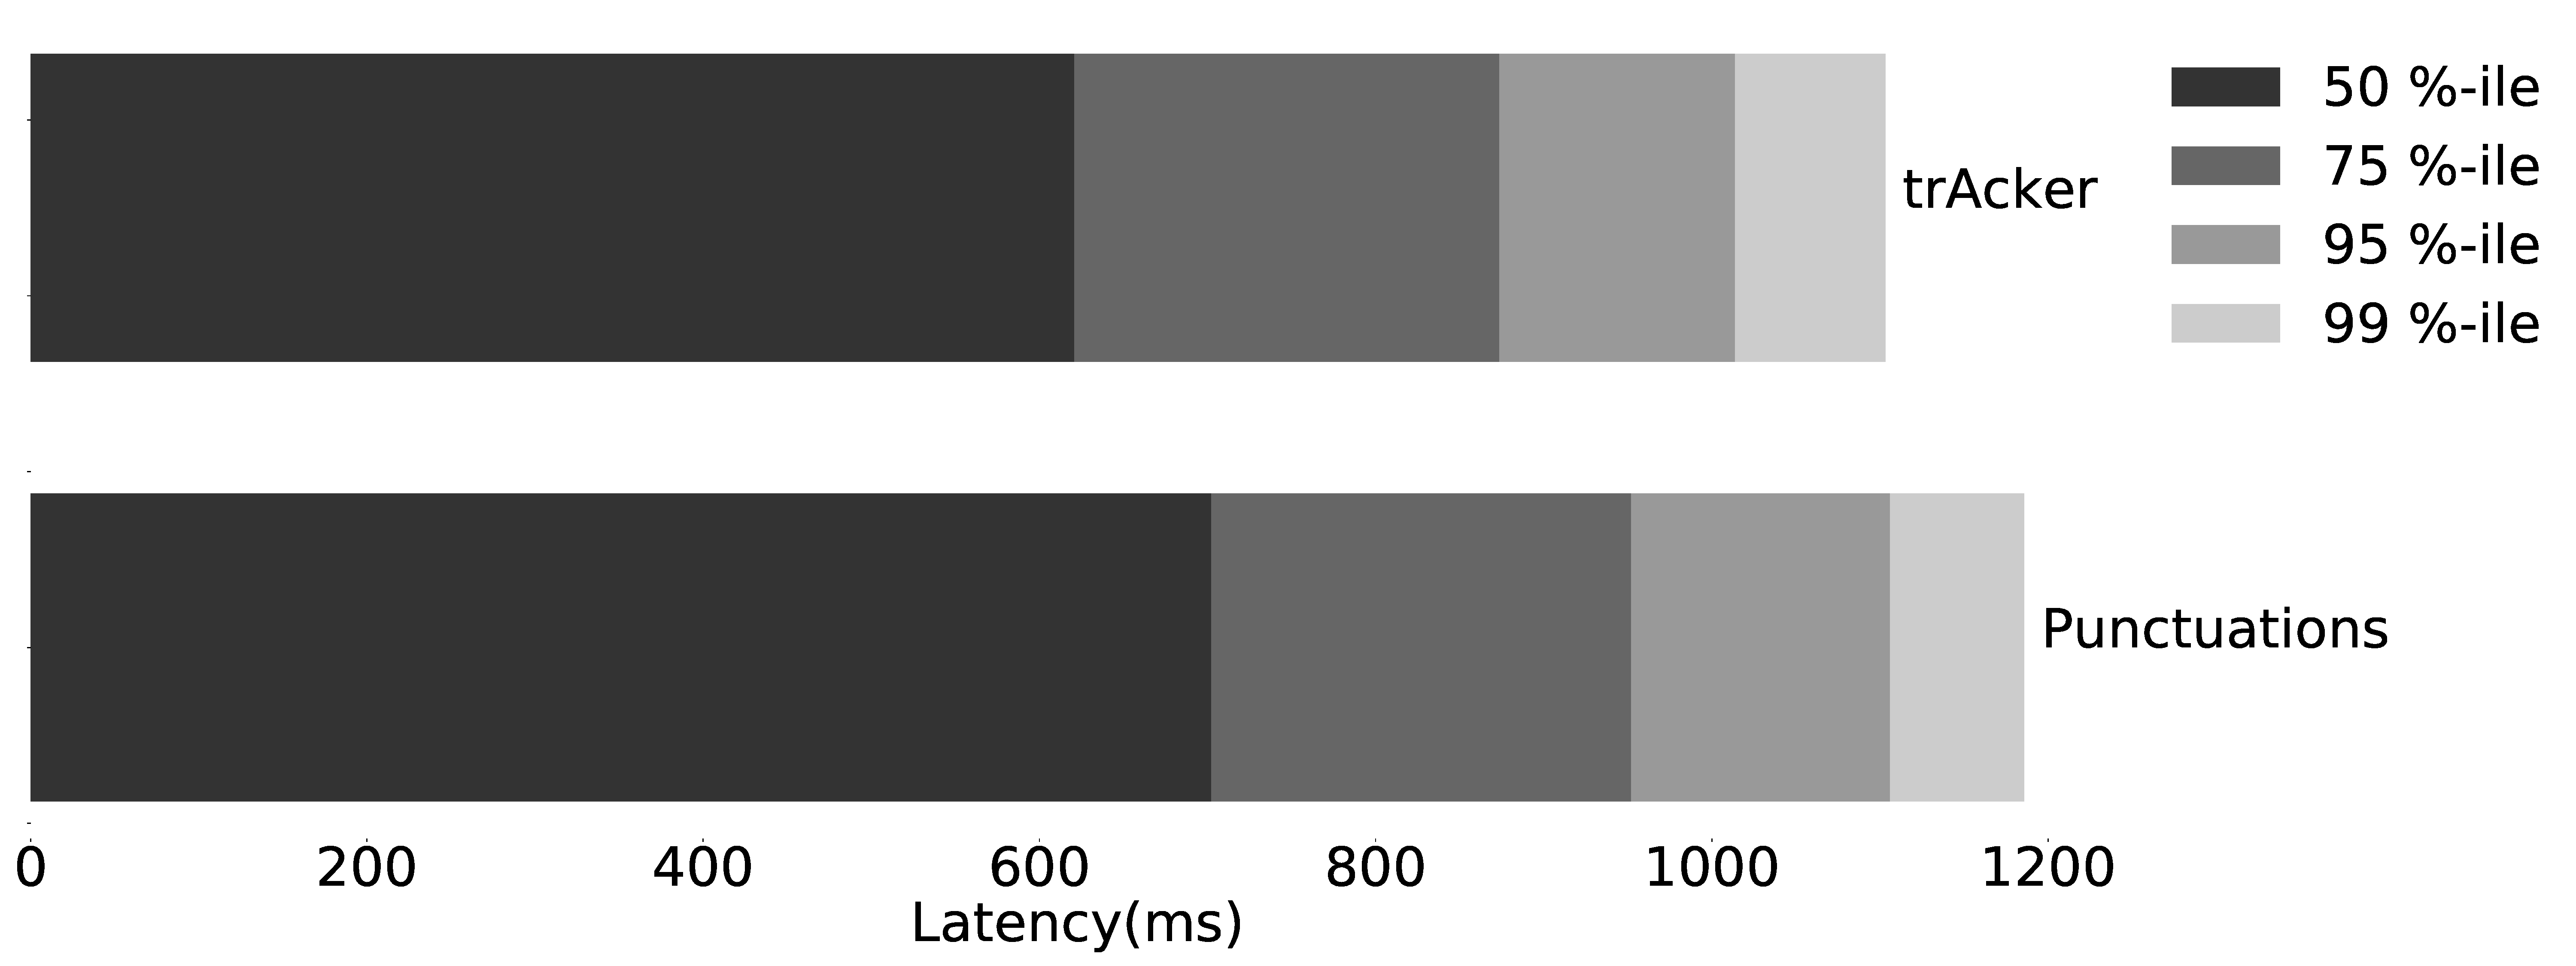
\includegraphics[width=0.99\textwidth]{pics/buffering_latencies_barh_1000.pdf}
%             \caption{1000 ms snapshot duration}
%             \label{1000ms_snapshot}
%     \end{subfigure}
%     \caption{Latency spikes during state snapshotting}
%     \label{snapshot_spikes}
% \end{figure*}

% \subsection{State snapshotting} \label{snapshotting}

% As we mentioned above, another important application of dependency tracking mechanisms is state snapshotting. Typically, state snapshotting is implemented as follows: a streaming system divides input records into the contiguous parts called epochs. When an operator entirely processes all items from a particular epoch, it blocks all inputs and persistently saves its local state. Each operator can receive the notification and start to save its state independently from other operators. Hence, there is a need for operator-level dataflow locality of tracking. Flink~\cite{Carbone:2017:SMA:3137765.3137777}, Storm~\cite{apache:storm:state}, IBM Streams~\cite{jacques2016consistent}, and Heron~\cite{Kulkarni:2015:THS:2723372.2742788} implement this state snapshotting scheme. All these systems use marker-based techniques to provide notifications for operators.

% A dependency tracking mechanism can imply latency overhead on this protocol. In the case of markers, the overhead is caused by blocking an operator after the first marker is received and until the operator receives markers from all inputs. This behavior is known as {\em marker alignment} issue~\cite{Carbone:2017:SMA:3137765.3137777}. In the case of \tracker , an operator must buffer element from the next epoch until {\em MinTimeUpdate} for the previous epoch is received.

% % https://gist.github.com/faucct/6097d9d08197cb979b71721b16f8b6a3/
% \begin{figure}[htbp]
%   \centering
%   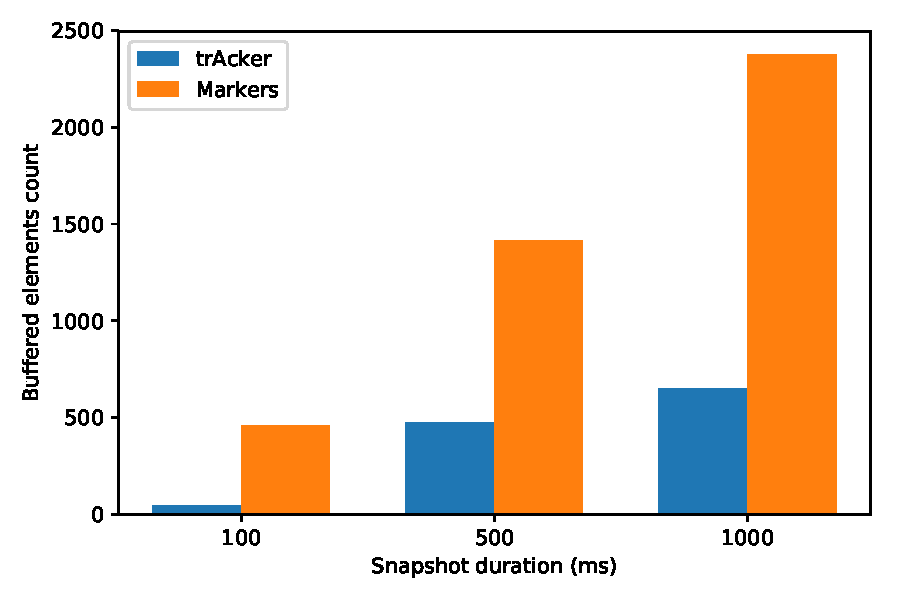
\includegraphics[width=0.50\textwidth]{pics/buffering_count_bars.pdf}
%   \caption{Buffered elements count}
%   \label{snapshot_buffered}
% \end{figure}

% Figure~\ref{snapshot_spikes} demonstrates latency spikes during state snapshotting for markers and \tracker , depending on the persistent save duration. In general, \tracker\ provides 50-120 milliseconds fewer latency spikes. This difference can be significant for latency-conscious applications~\cite{zhang2017sub}. The low notification latency explains this difference, as we demonstrated in Section~\ref{completeness}. Low notification latency leads to a smaller number of elements that need to wait (be buffered), as it is shown if Figure~\ref{snapshot_buffered}. The smaller number of buffered records causes lower buffering duration that implies lower spikes in general. Note, the vast difference in the number of buffered elements does not necessarily imply the vast difference in total buffering duration because most of the buffered elements wait for a tiny amount of time.

% This experiment indicates that \tracker\ can provide better results for a common problem that is traditionally solved using markers. This result also shows that operator-level locality of tracking can be implemented efficiently with \tracker .

% \begin{figure}[htbp]
%   \centering
%   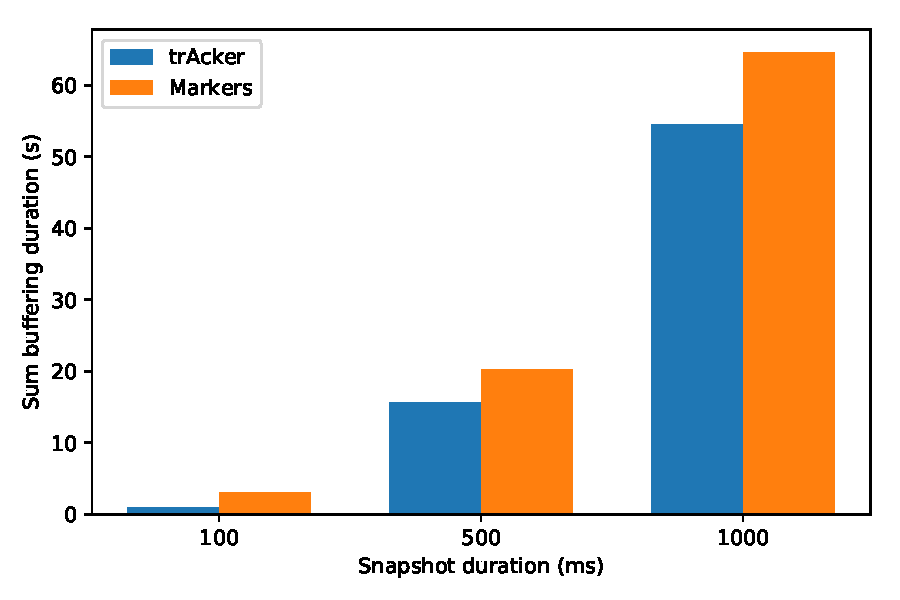
\includegraphics[width=0.50\textwidth]{pics/buffering_sum_duration_bars.pdf}
%   \caption{Total buffering duration}
% \end{figure}


\section{Related Work}
\label {fs-acker-related}

Many state-of-the-art SPEs adapt punctuations for various substream management problems. Flink~\cite{Carbone:2017:SMA:3137765.3137777}, Storm~\cite{Toshniwal:2014:STO:2588555.2595641}, Samza~\cite{Noghabi:2017:SSS:3137765.3137770} apply punctuations for both window aggregations and state snapshotting problems. MillWheel~\cite{Akidau:2013:MFS:2536222.2536229} has another state management model but also uses punctuations as a window end indicator. Spark Streaming~\cite{Zaharia:2012:DSE:2342763.2342773} method for state clean-up bases on punctuations as well.

Several techniques are aimed at solving the particular problems but do not provide the general substream management framework. Apache Storm {\em Acker}~\cite{apache:storm:acker} is a method for completeness monitoring: it allows SPE to detect if some element has been lost during the processing. Naiad~\cite{Murray:2013:NTD:2517349.2522738} uses a kind of similar to \tracker\ mechanism for tracking the progress of iterative computations. Another technique for tracking iterations it introduced in~\cite{chandramouli2014trill}.

Another related research direction is the generation of substream termination signals from data producers. Some systems apply periodic scheme~\cite{Akidau:2013:MFS:2536222.2536229, Akidau:2015:DMP:2824032.2824076}, while others try to use knowledge about the content of the data. Adaptive approch~\cite{awad2019adaptive} does not use any information about data but takes into account arrival rate and delay. The enhancements of these methods can increase the applicability of substream management in practice.

% Most dependency tracking techniques employed in state-of-the-art stream processing systems are discussed in detail in Section~\ref{existing_solutions}. In this section we hightlight the differences between 

% Naiad~\cite{Murray:2013:NTD:2517349.2522738} uses a kind of similar to \tracker\ mechanism for tracking the progress of iterative computations. Within this method, each data item in a system is assigned with an {\em epoch} and a vector of logical timestamps called {\em loop counter}. Epoch is similar to our notion of {\em global time} concept but provided by an external user. The value on the $i$th position of the loop counter indicates the number of times this element went through the $i$th {\em loop context} (cycle) in a dataflow. Special distributed agents monitor for the items and their timestamps and notify when all elements reach some iteration number or all elements from an epoch are entirely processed. There are three main differences between the mentioned technique and the \tracker. Firstly, \tracker\ relies on the global identifier of an element provided by a system itself. Secondly, the protocol used in Naiad causes the enormous number of extra network messages that quadratically depend on the number of machines even with optimizations~\cite{Murray:2013:NTD:2517349.2522738}. Thirdly, Naiad's method uses counter updates (+1/-1) instead of XORs, hence update messages do not commutate. This fact complicates the implementation (especially distributed) of this method.

% The problems of transactional processing, providing for delivery guarantees, and fault tolerance, are extensively studied in recent years~\cite{Akidau:2013:MFS:2536222.2536229, Carbone:2017:SMA:3137765.3137777, thepaper, Wang:2019:LSF:3341301.3359653}. While state-of-the-art stream processing systems still provide high overhead on regular processing due to fault tolerance protocols, transactional processing, etc., we expect that this area will be studied further. As we mentioned above, a dependency tracking mechanism is an essential part of the solutions to these problems. Hence, \tracker\ can be applied to optimize the existing techniques.

\section {Conclusion}
\label {fs-acker-conclusion}

% In this work, we formulated a problem of dependency tracking between input and output elements in streaming dataflows. We demonstrated that state-of-the-art distributed stream processing systems face this problem in state snapshotting mechanisms~\cite{Carbone:2017:SMA:3137765.3137777, apache:storm}, the materialization of time-varying relations~\cite{Begoli:2019:OSR:3299869.3314040}, and atomic delivery of all descendants of an input item~\cite{we2018adbis}.  

% To solve this problem, we proposed a mechanism that adopts ideas from the Apache Storm completion tracking mechanism called \acker. We extend each data item with a logical timestamp that denotes corresponding input items and tracks if dataflow contains elements with specific timestamps. 

% Our solution, called \tracker\ inherits from \acker\ fine-grained tracking, and cyclic dataflows support and provides the following features:
% \begin{itemize}
%     \item {\bf Notifications order preservation:} the order of notifications that system completely processed some set of input items does not contradict the order of input elements. This feature allows using \tracker\ for state snapshotting.
%     \item {\bf Dataflow locality:} different parts of a dataflow can receive independent notifications that allow a stream processing system to apply efficient asynchronous state snapshotting algorithms, e.g., one that is used in Apache Flink~\cite{Carbone:2017:SMA:3137765.3137777}. 
%     \item {\bf Scalability:} we introduced a distributed version of \tracker\ that allows a system to distribute extra network traffic between all computational units. 
%     \item {\bf Low overhead:} \tracker\ does not produce any significant performance penalty and does not affect the throughput of a distributed streaming dataflow.
% \end{itemize}

% We conducted a series of experiments and compared the proposed method with a baseline approach based on the markers mechanism used in Apache Flink. We demonstrated that both centralized and decentralized implementations of \tracker\ provide lower notification latency that does not considerably degrade with an increase of a logical graph size or a cluster size. Experiments also showed that \tracker\ has lower throughput overhead in case of fine-grained tracking.

In this work, we formalized the problem of substreams management and demonstrated the main properties of the most common punctuations approach that bases on injecting special elements (punctuations) into the stream. On the one hand, receiving such elements naturally guarantees the end of a substream since that moment, because all elements within the operator are totally ordered. On the other hand, propagating punctuations through a whole dataflow leads to the lack of cyclic dataflows support, poor scalability, and excessive extra traffic.

We designed and implemented a new substreams management technique called \tracker\ that does not require injecting service elements directly into the stream. Instead, we mark all data elements with ordered labels and designed the distributed agent, which notifies operators that a substream ends since receiving an input element with the specified label. Our approach provides the following features:

\begin{itemize}
     \item {\bf Cyclic dataflows support:} the method is suitable for problems that require non-linear executions: graph traversing, iterative algorithms, etc. We evaluated this feature within the real-life problem.
     \item {\bf Low overhead:} we showed that our implementation implies a lower amount of extra network traffic. We demonstrated that it produces low performance penalty, and insignificantly affects the throughput of SPE.
     \item {\bf Better scalability:} extra network traffic from operators can be distributed between multiple nodes. Experiments on synthetic dataflows indicated the practical feasibility of balancing extra traffic.
\end{itemize}



% both centralized and decentralized implementations of \tracker\ provide lower notification latency that does not considerably degrade with an increase of a logical graph size or a cluster size. Experiments also showed that \tracker\ has lower throughput overhead in case of fine-grained tracking.

% \appendix 
% \section {Punctuations} \label{appendix:punctuations-proof}
% \section {\tracker} \label{appendix:tracker-proof}

\bibliographystyle{ACM-Reference-Format}
% \bibliography{bibliography/flame-stream}
\bibliography{bibliography/flame-stream}

\end {document}

\endinput
